\setbeamercovered{transparent}
\section{Netzwerktopologie und Dynamik}
\newcommand{\mdeg}{\bar{k}}
\newcommand{\vertices}{V}
\newcommand{\initrand}{\emph{init\_random\_weight}}
\newcommand{\infparamrand}{\emph{random\_infection\_parameters}}
\newcommand{\poprand}{\emph{random\_population}}
\newcommand{\medges}{\bar{L}}
\begin{frame}[t]{Netzwerktopologien} 
    Verschiedene Modelle zur Erzeugung von zufälligen Netzwerken:
    \begin{itemize}
        \item<1> Erdos-Renyi
            \begin{itemize}
            \item Parameter:
                \begin{itemize}
                    \item Anzahl der Knoten $\vertices$ (\emph{num\_vertices})
                    \item Mittlere Kantenanzahl $\mdeg$ (\emph{mean\_degree})
                \end{itemize}
            \item $p_k \sim Bin(N, k)$
            \item $\medges = \frac{\vertices \mdeg}{2}$
            \item Small World Eigenschaft
        \end{itemize}
        \item<2-> Bollobas-Riordan
            \begin{itemize}
                \item Skalenfreies Netzwerk: $p_k \sim k^{-\gamma}$
                \item Momente $<k^{\gamma -1}>$ größer $\gamma - 1$ von $p_k$ sind nicht endlich
                \item Parameter:
                    \begin{itemize}
                        \item $\alpha = 0.2, \beta=0.8, \gamma = 0., \delta_{in} = 0.,
                            \delta_{out} = 0.5$
                    \end{itemize}
            \end{itemize}
    \end{itemize}
    In Utopia sind Netzwerkgeneratoren über Boost Graph Library implementiert.
\end{frame}
\begin{frame}{Zusätzliche Eigenschaften}
    \begin{itemize}
        \item Initialisierung der Population auf Knoten 
            \begin{itemize}
                \item Standard: Exponentiell verteilte Population
            \end{itemize}
        \vfill\item<2-> Kantengewichte:
            \begin{itemize}
                \item Zufälliges Gewicht $w_{ij} = [0,$ \emph{init\_weight}$]$
                \item Standard: \emph{init\_weight}$=0.01$
            \end{itemize}
        \vfill\item<3-> Randomisierung der Infektionsparameter auf Knoten
            \begin{itemize}
                \item Standard: $\beta$ randomisiert
            \end{itemize}
    \end{itemize}
\end{frame}

\subsection{Erdos-Renyi}
\begin{frame}[t]
    \frametitle{Erdos-Renyi: Netzwerk}
    \begin{figure}[htpb]
        \centering
        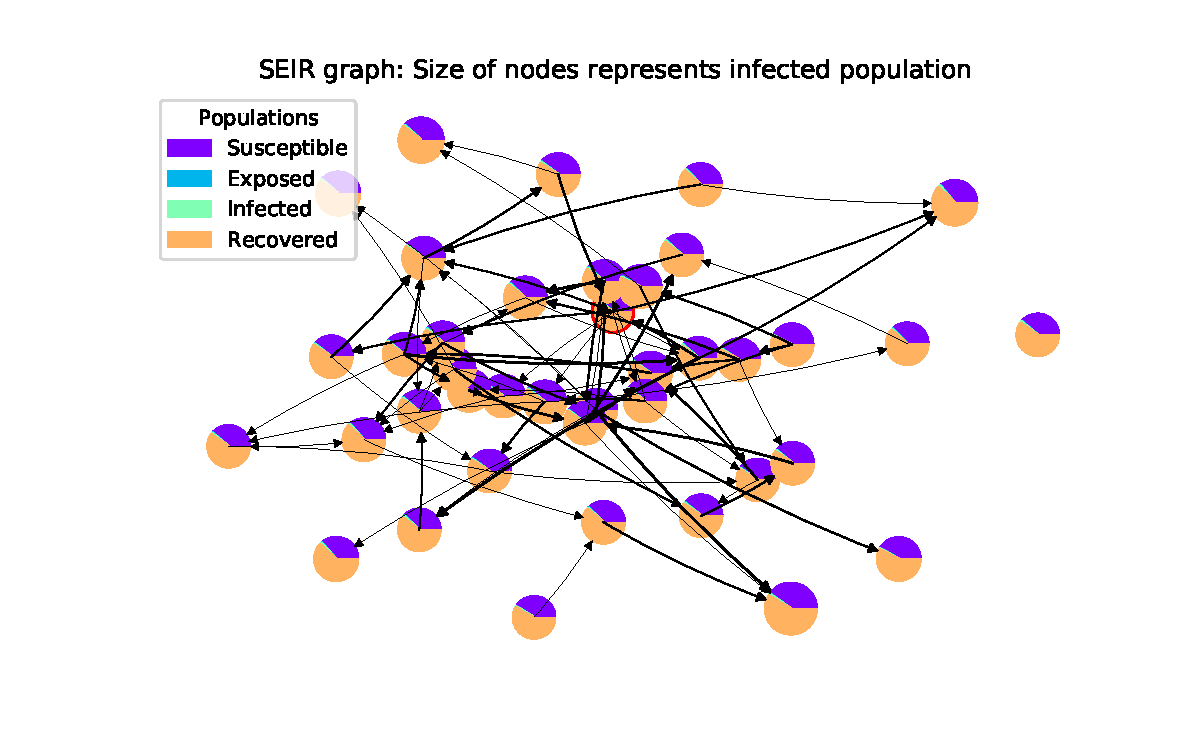
\includegraphics[width=0.8\linewidth]{ER_migration_network_40-2.pdf}
        \caption{Erdos-Renyi Netzwerk mit $\vertices = 40, \mdeg = 2$ für den letzten
        simulierten Zeitpunkt ($t= 10^{4}$)}%
        \label{fig:ER_migration_network_40-2}
    \end{figure}
\end{frame}
\begin{frame}[c]
    \frametitle{Erdos-Renyi: Netzwerkdynamik}
    Simulation: \href{run:/figures/animations/ER_animation_40-2.mp4}{Erdos-Renyi Derivative Network Animation}
\end{frame}
\begin{frame}[t]
    \frametitle{Erdos-Renyi: Knotenanzahl}
    Gesamtpopulation für variierte Knotenanzahl $\vertices = 12, 100$: 
    \begin{columns}
        \begin{column}{0.5\textwidth}
    \begin{figure}[htpb]
        \centering
        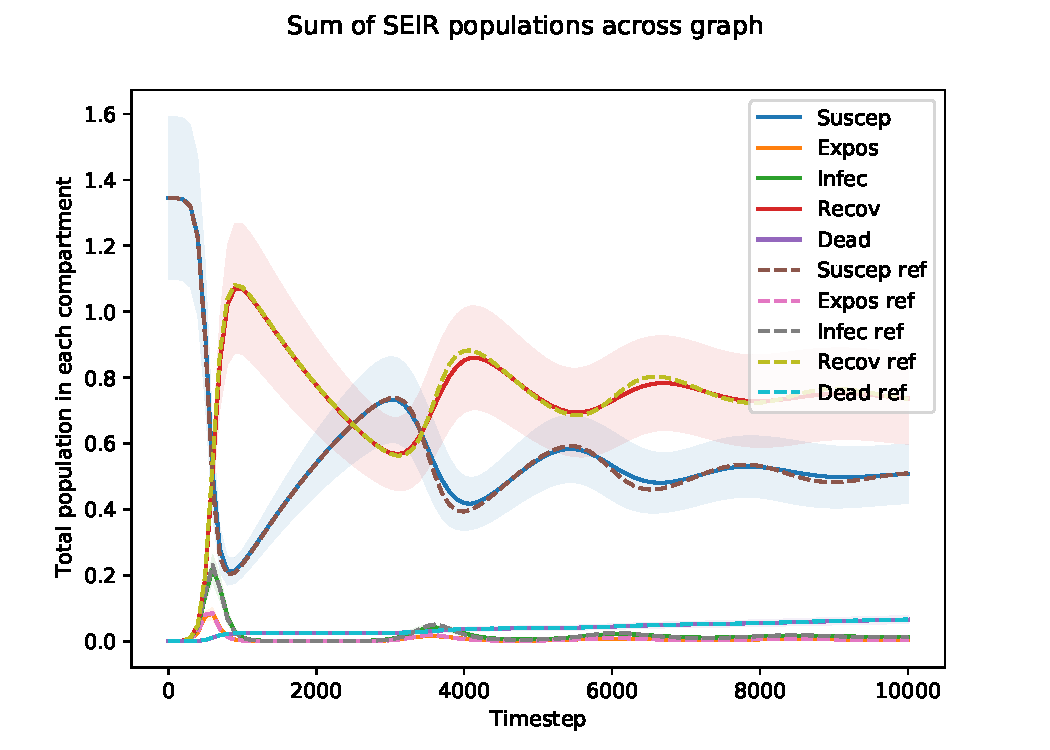
\includegraphics[width=1\linewidth]{E_vert12_mdeg2_totpop.pdf}
        \caption{Knotenanzahl $\vertices=12$ und mittlere Kantenzahl $\mdeg = 2$.
        Standardeinstellungen.}%
        \label{fig:E_vert12_mdeg2_totpop}
    \end{figure}
\end{column}
\begin{column}{0.5\textwidth}
    \begin{figure}[htpb]
        \centering
        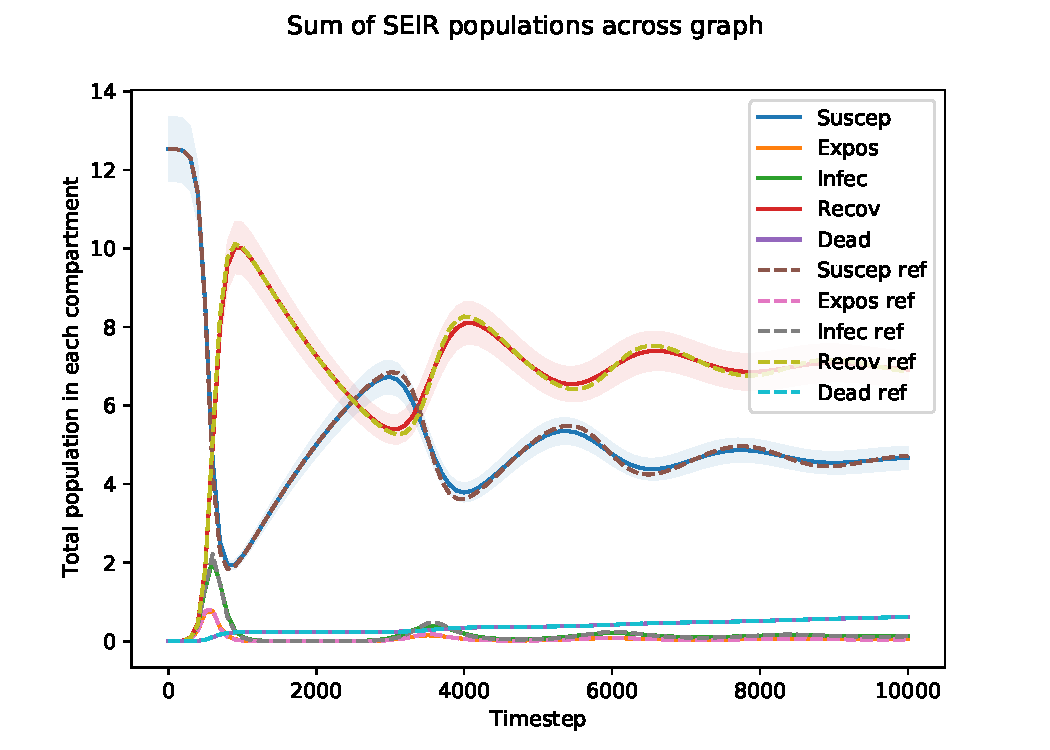
\includegraphics[width=1\linewidth]{ERs_totpop_100-2.pdf}
        \caption{Knotenanzahl $\vertices=100$ und mittlere Kantenzahl $\mdeg = 2$.
        Standardeinstellungen.}%
        \label{fig:ERs_totpop_100-2-a}
    \end{figure}
\end{column}
\end{columns}
\begin{itemize}
    \item Geringfügig bessere Übereinstimmung mit dem Referenzmodell für höhere $\vertices$
    \item Höhere Robustheit gegenüber Seed
\end{itemize}
\end{frame}
\begin{frame}[t]
    \frametitle{Erdos-Renyi: Knotenanzahl}
    Prozentuale Abweichung der Infektionswellen (Sim/Ref)
    \begin{figure}[htpb]
        \centering
        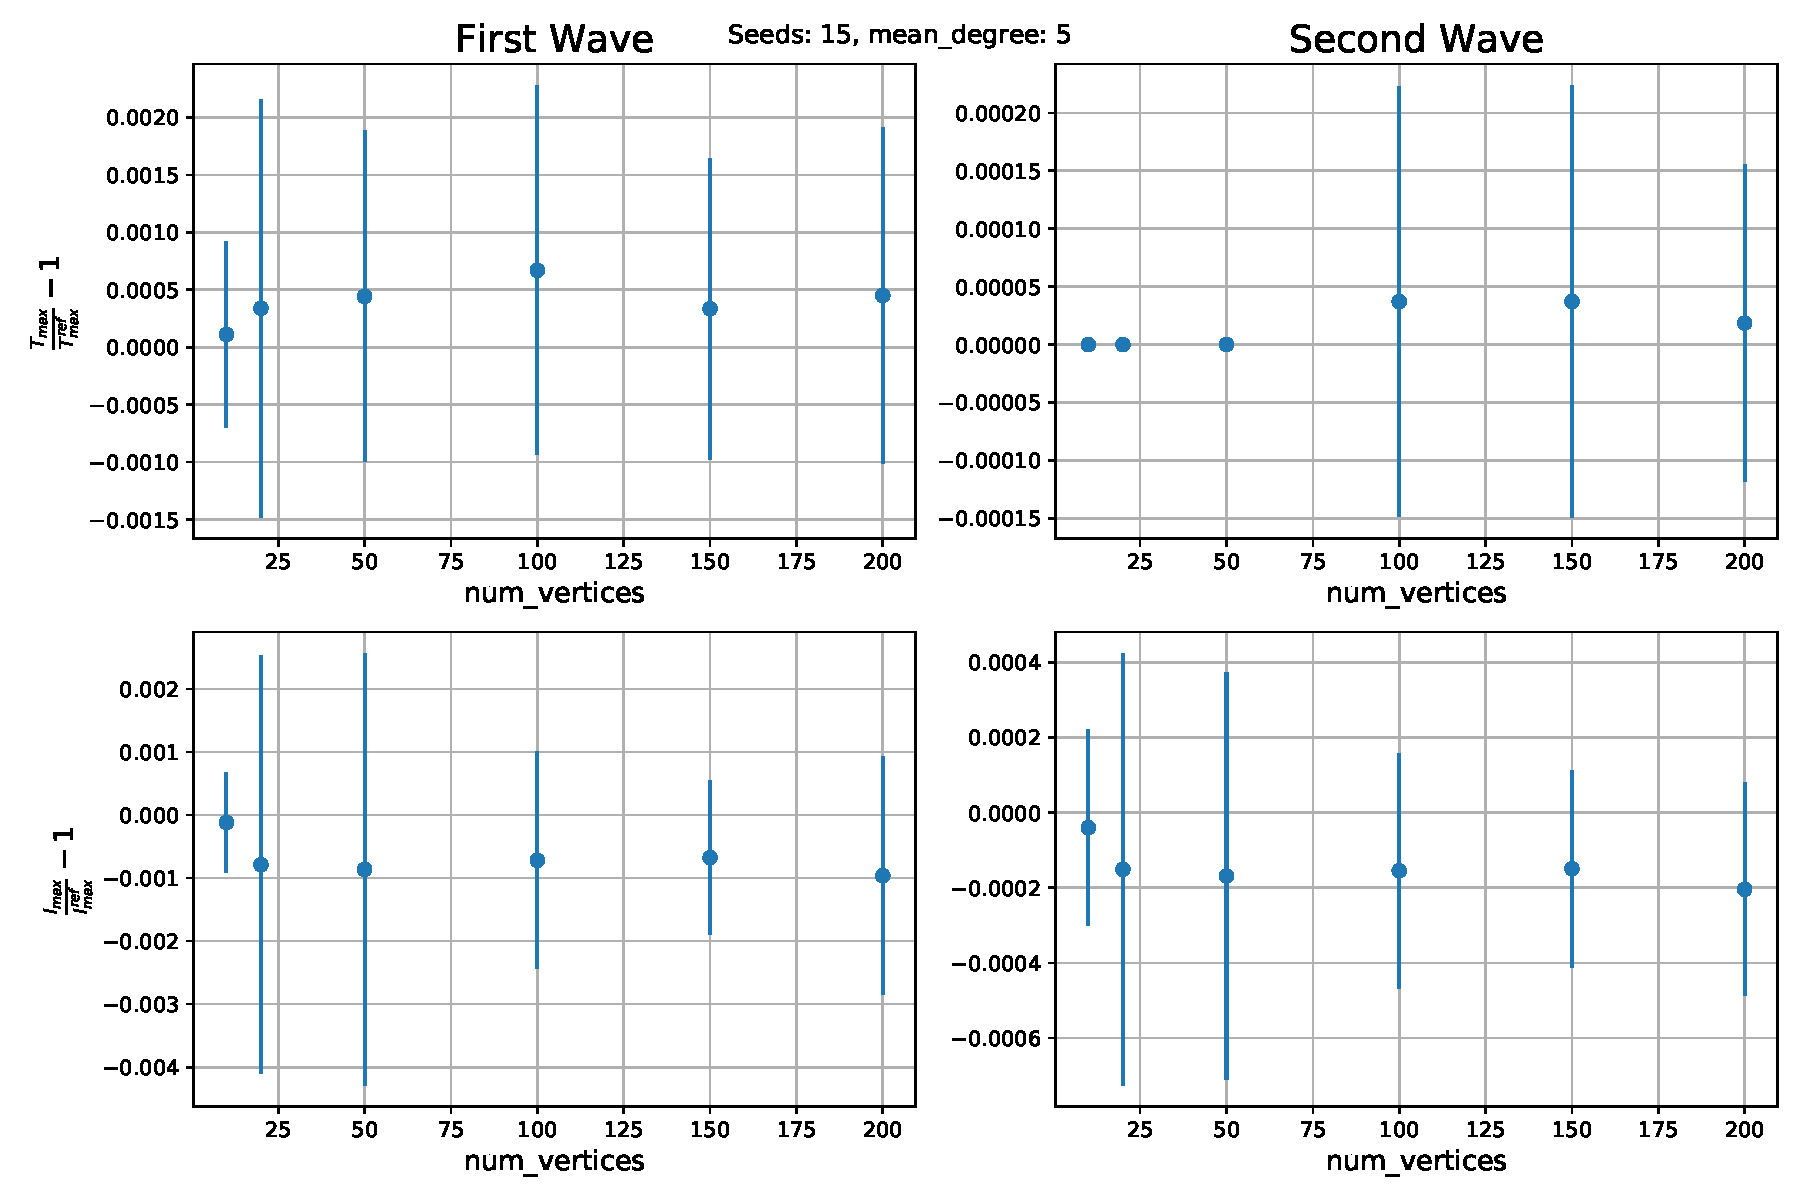
\includegraphics[width=0.8\linewidth]{ERs_swvert_finf_rinits_rpop-wavecomp.pdf}
        \caption{Fehlerbalken: Zweifache Standardabweichung. $\mdeg = 5$. Fixe Infektionsparameter, sonst Standardeinstellungen.}%
        \label{fig:ERs_swvert_finf_rinits_rpop-wavecomp}
    \end{figure}


\end{frame}
\begin{frame}[t]
    \frametitle{Erdos-Renyi: Mittlere Kantenzahl}
    Gesamtpopulation für konstantes $\vertices = 12$ aber $\mdeg = \{2, 6\}$
    \begin{columns}
        \begin{column}{0.5\textwidth}
            \begin{figure}[htpb]
                \centering
                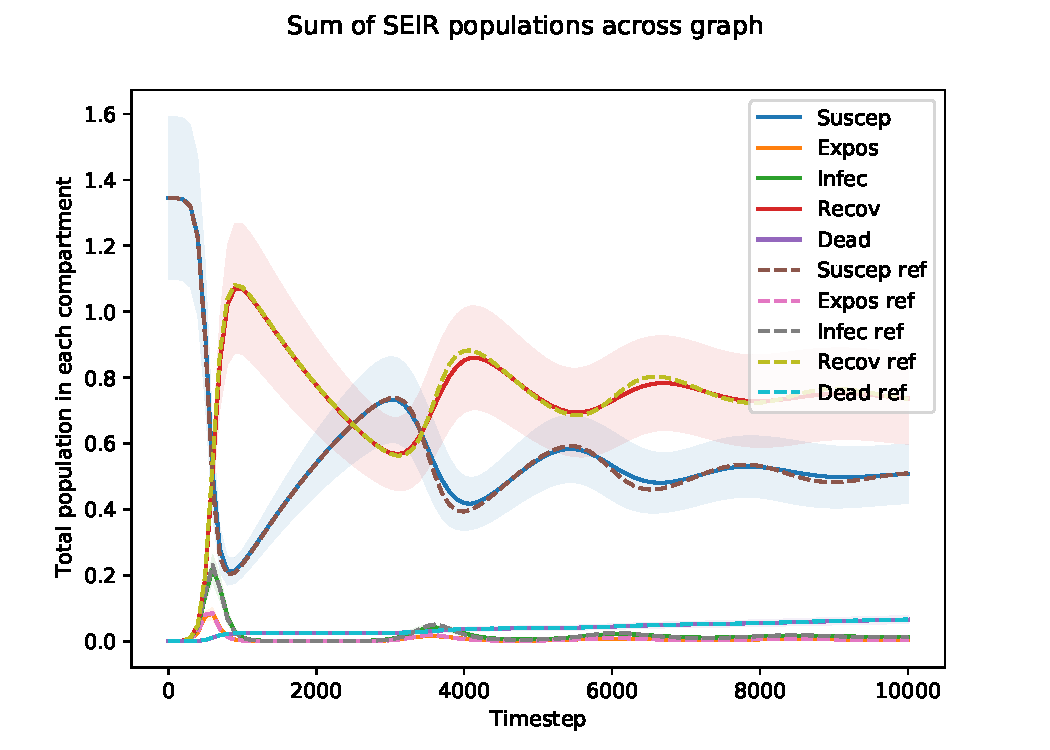
\includegraphics[width=1\linewidth]{ERs_totpop_12-2.pdf}
                \caption{$\mdeg = 2$, Standardeinstellungen.}
                \label{fig:ERs_totpop_12-2}
            \end{figure}
        \end{column}
        \begin{column}{0.5\textwidth}
            \begin{figure}[htpb]
                \centering
                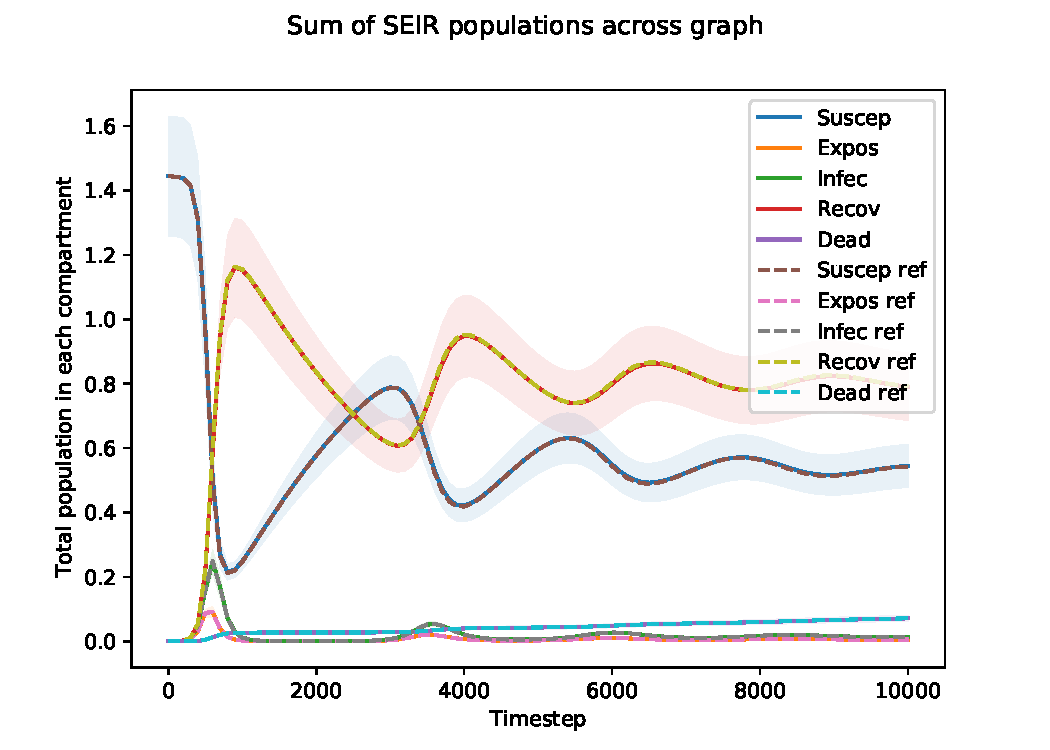
\includegraphics[width=1\linewidth]{ERs_totpop_12-6.pdf}
                \caption{$\mdeg = 6$, Standardeinstellungen.}
                \label{fig:ERs_totpop_12-6}
            \end{figure}
        \end{column}
    \end{columns}
    \begin{itemize}
        \item Höheres $\mdeg$ reduziert Abweichung zu Referenzmodell
        \item Robustheit gegenüber Seed ist erhöht
    \end{itemize}
\end{frame}

\begin{frame}[t]
    \frametitle{Erdos-Renyi: Mittlere Kantenzahl}
    Prozentuale Abweichung der Infektionswellen (Sim/Ref)
    \begin{figure}[htpb]
        \centering
        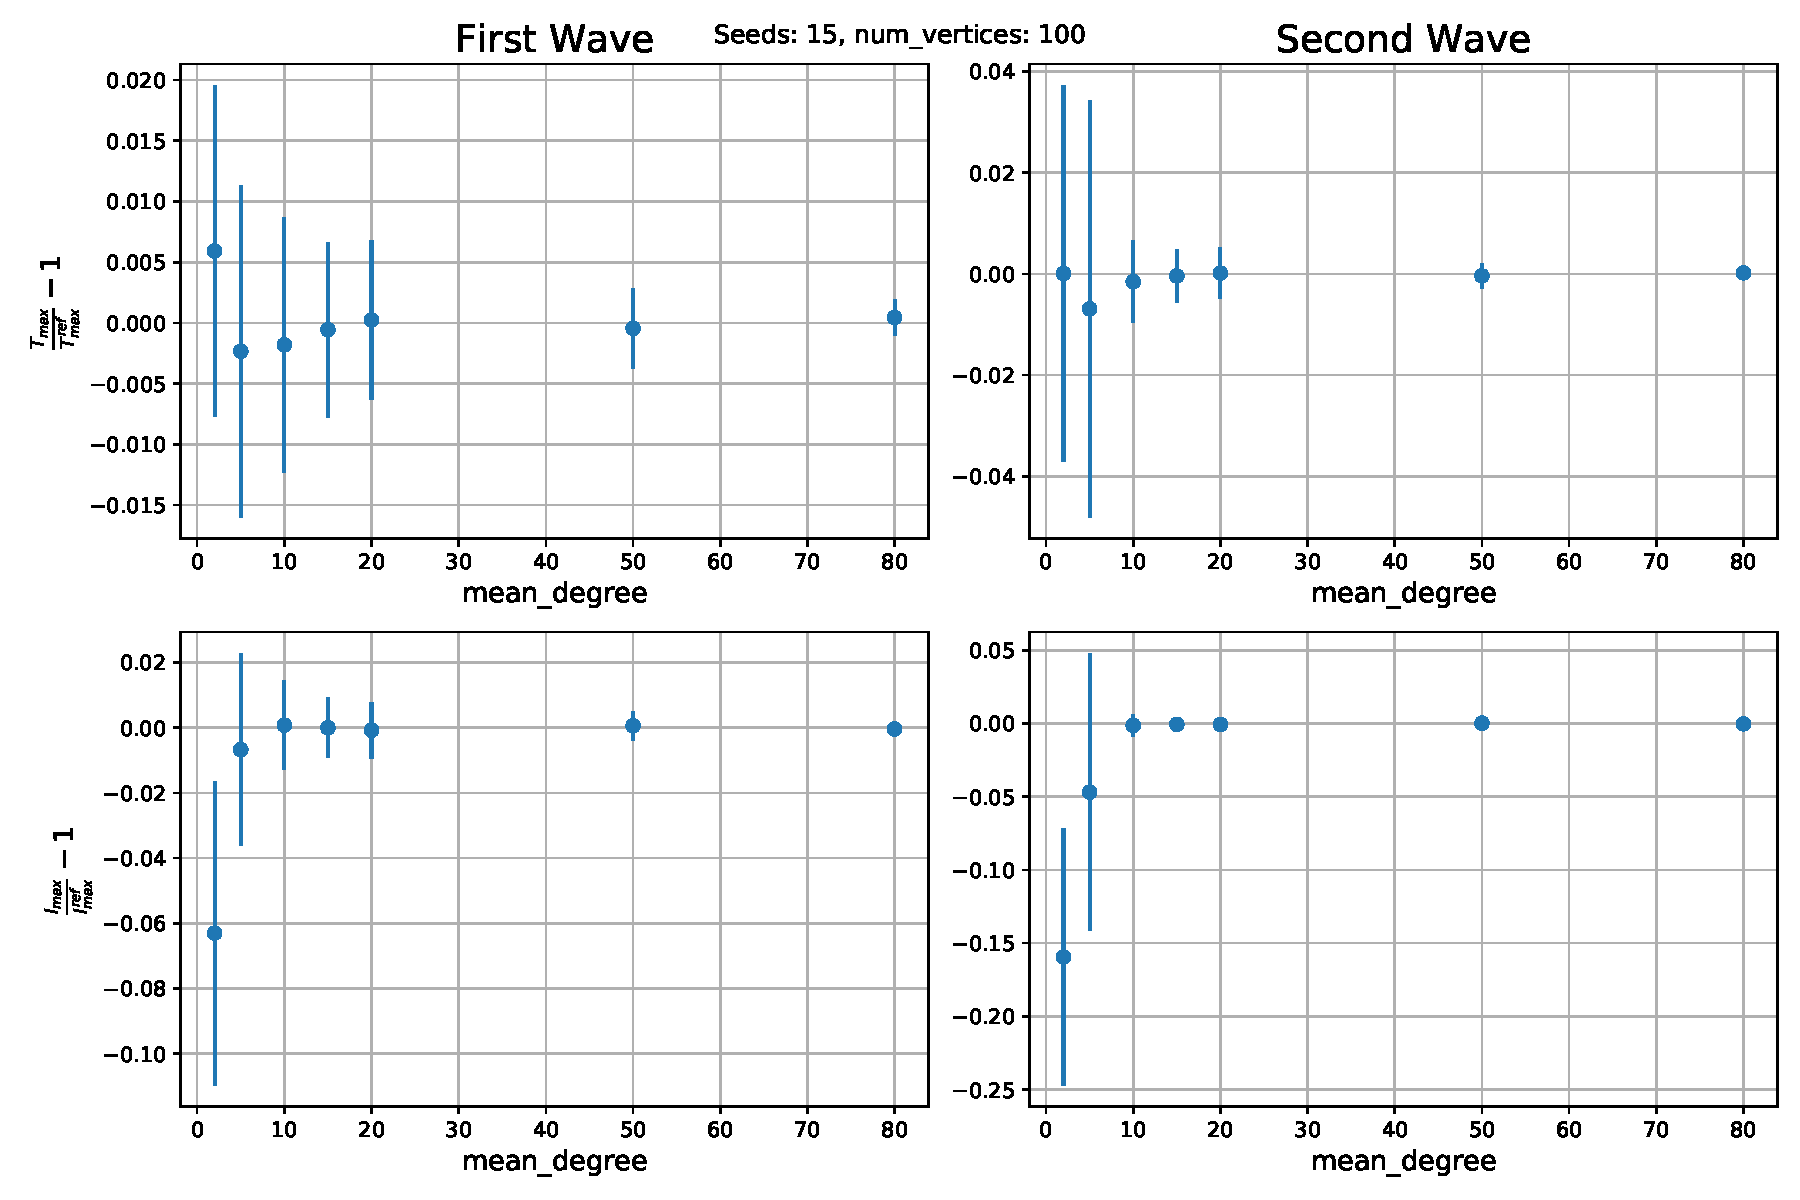
\includegraphics[width=0.8\linewidth]{ERs_swmdeg_rinf_rinits_rpop-wavecomp.pdf}
        \caption{Fehlerbalken: Zweifache Standardabweichung. $\vertices = 100$. Standardeinstellungen.}%
        \label{fig:ERs_swmean_finf_rinit_rpop-wavecomp}
    \end{figure}
\end{frame}
\begin{frame}[t]
    Vergleich der ersten Infektionswelle für verschiedene Seeds
    \frametitle{Erdos-Renyi: Mittlere Kantenzahl}
    \begin{figure}[htpb]
        \centering
        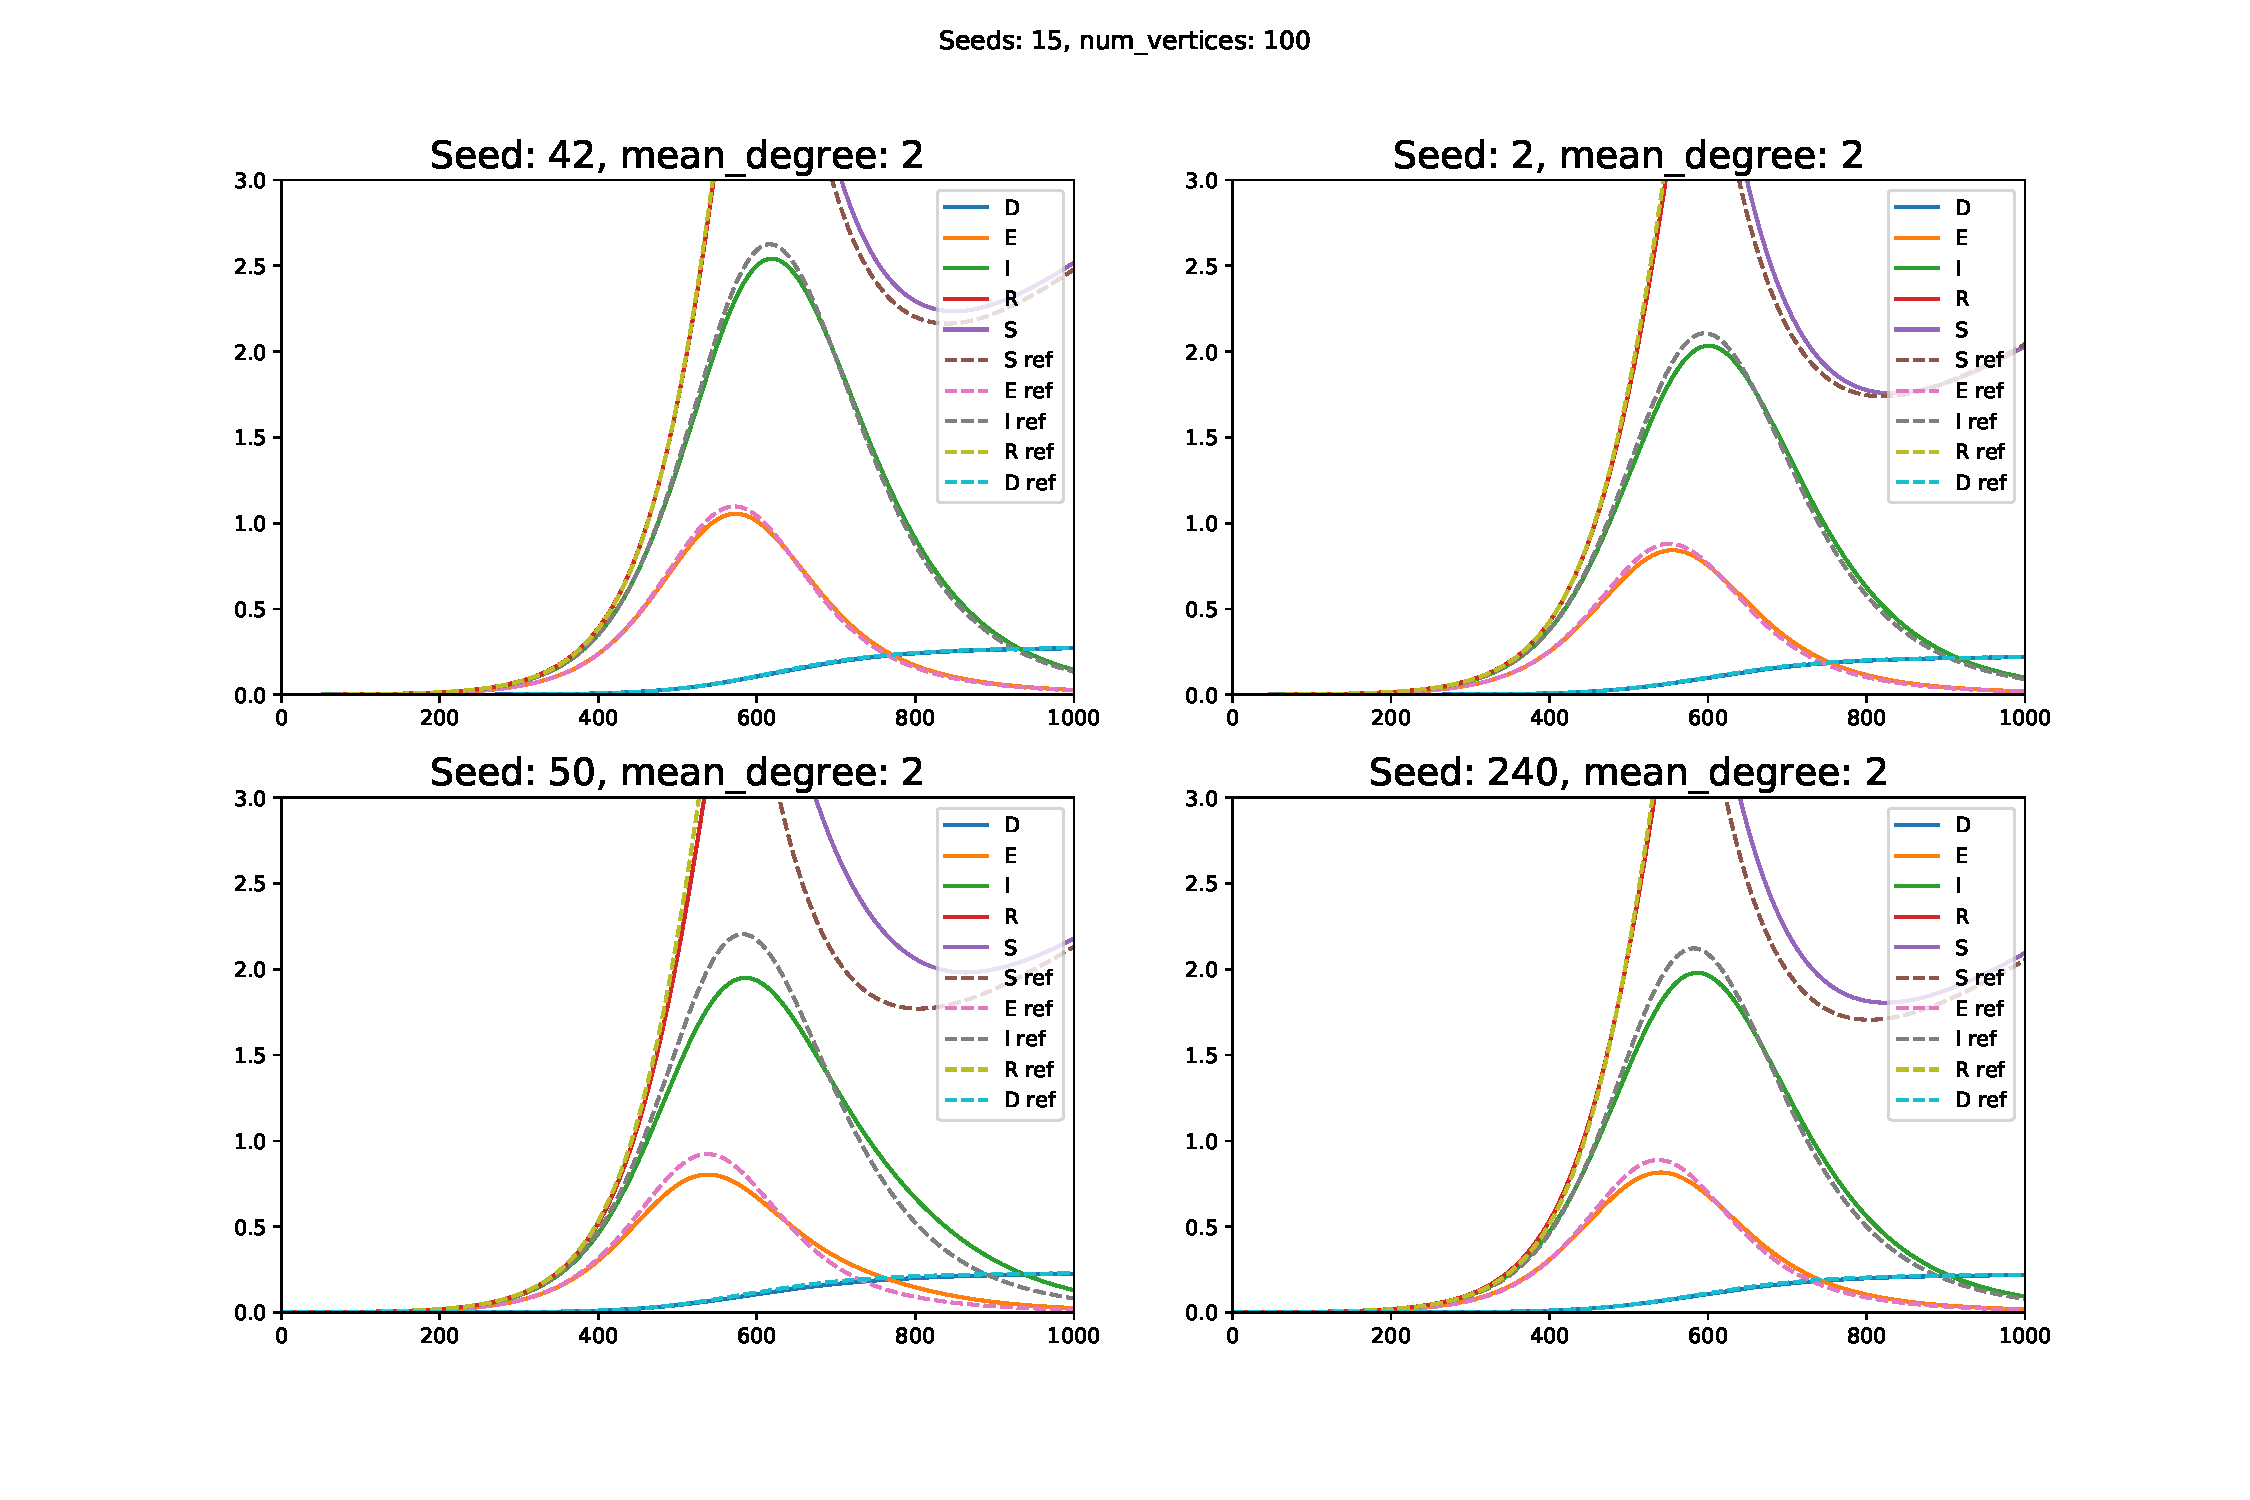
\includegraphics[width=0.8\linewidth]{ERs_swmdeg_rinf_rinits_rpop-seedcomp.pdf}
        \caption{Darstellung der ersten Infektionswelle aus dem Gesamtpopulationsplot. $\vertices = 100, \mdeg=2$.
        Standardeinstellungen.}%
        \label{fig:ERs_swmdeg_rinf_rinits_rpop-seedcomp}
    \end{figure}
\end{frame}

\subsection{Bollobas-Riordan}
\begin{frame}[t]
    \frametitle{Bollobas-Riordan: Netzwerk}
    \begin{figure}[htpb]
        \centering
        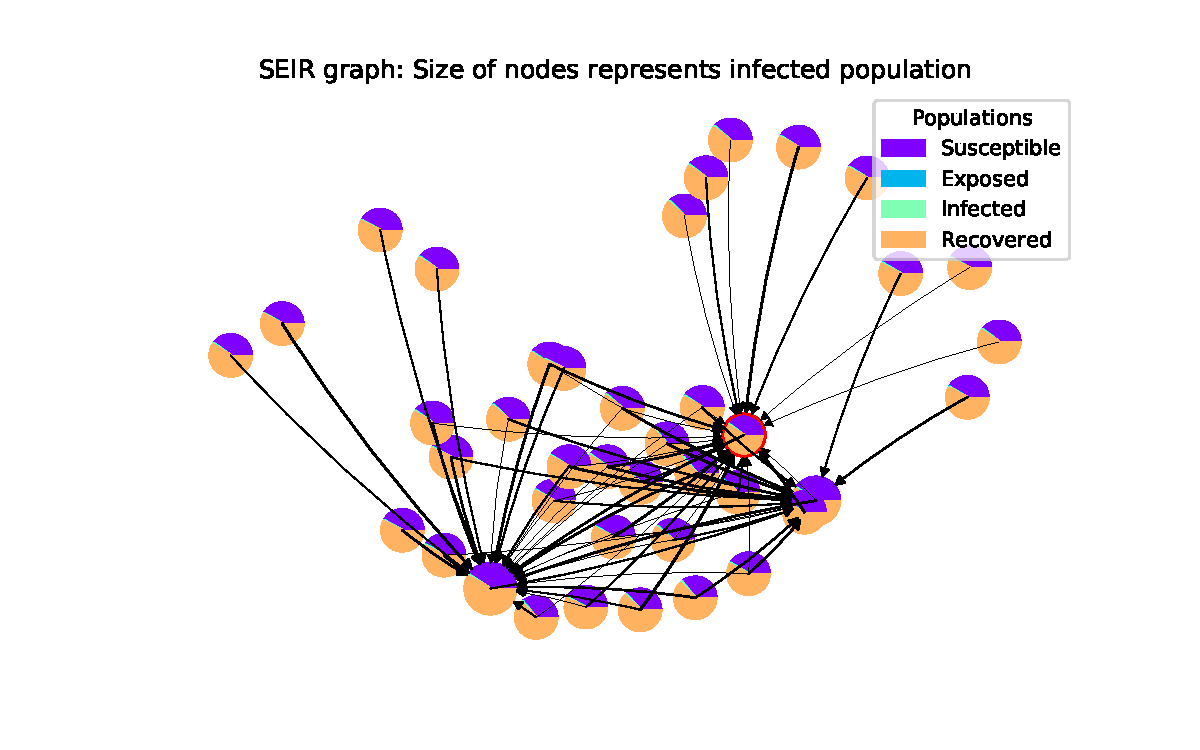
\includegraphics[width=0.8\linewidth]{BR_migration_network_40-2.pdf}
        \caption{Bollobas-Riordan Netzwerk mit $\vertices = 40, \mdeg = 2$ für den letzten
        simulierten Zeitpunkt ($t= 10^{4}$)}%
        \label{fig:BR_migration_network_40-2}
    \end{figure}
\end{frame}
\begin{frame}[c]
    \frametitle{Bollobas-Riordan: Netzwerkdynamik}
    Simulation: \href{run:/figures/animations/BR_animation_40-2.mp4}{Bollobas-Riordan Derivative Network Animation}
\end{frame}
\begin{frame}[t]
    \frametitle{Bollobas-Riordan}
    \begin{figure}[htpb]
        \centering
        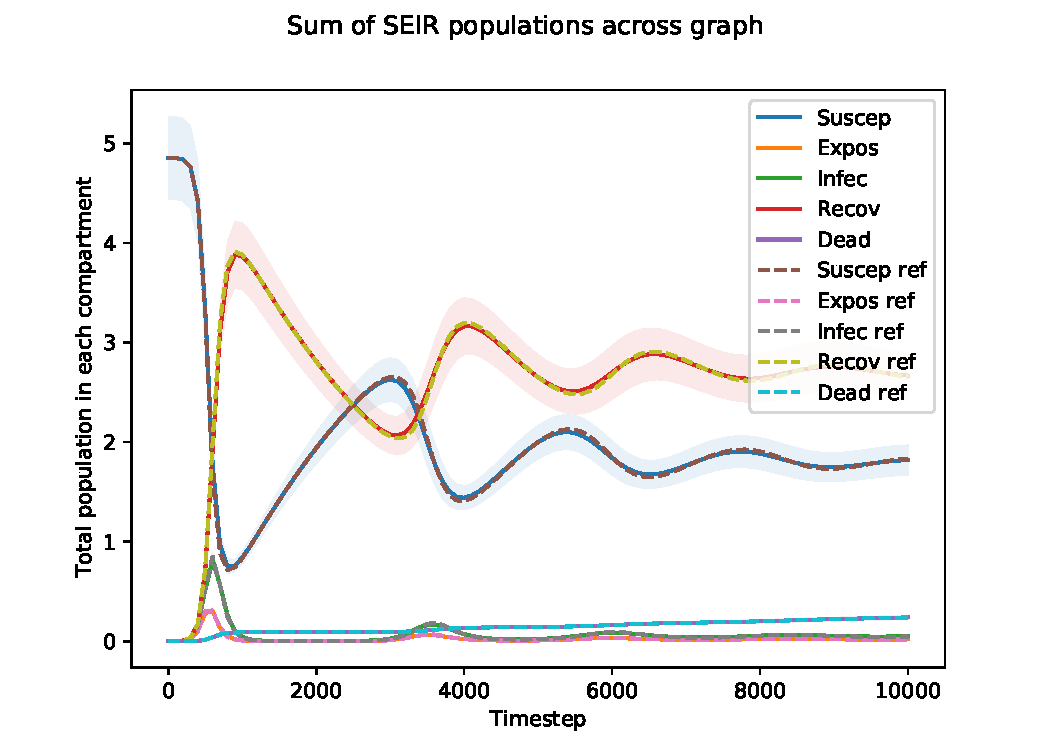
\includegraphics[width=0.8\linewidth]{Bs_totpop_40-2.pdf}
        \caption{Gesamtpopulation für $\vertices = 40$. Standardeinstellungen.}%
        \label{fig:Bs_totpop_40-2}
    \end{figure}
\end{frame}

\begin{frame}[t]
    \frametitle{Bollobas-Riordan: Knotenanzahl}
    Prozentuale Abweichung der Infektionswellen (Sim/Ref)
    \begin{figure}[htpb]
        \centering
            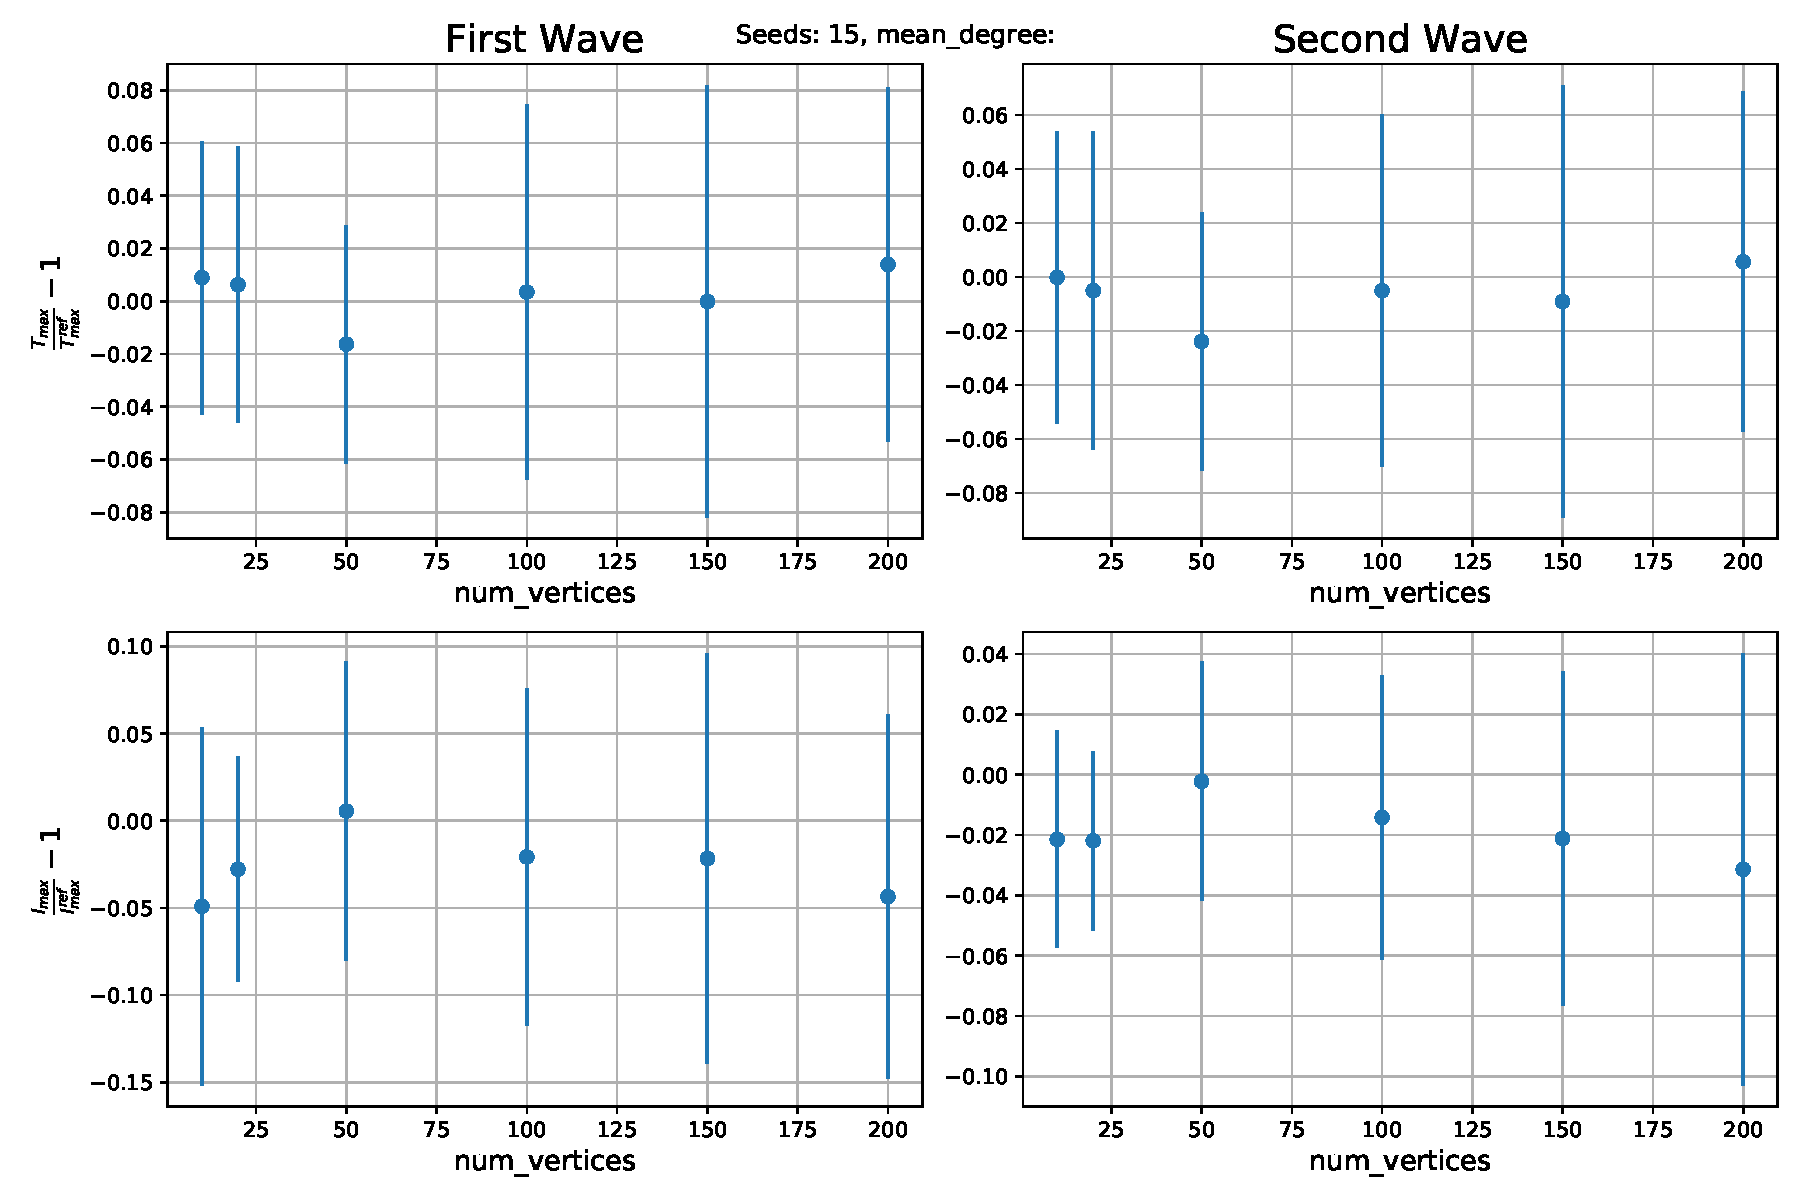
\includegraphics[width=0.8\linewidth]{Bs_swvert_rinf_rinits_rpop-wavecomp.pdf} \caption{Fehlerbalken: Zweifache Standardabweichung. Standardeinstellungen.}% 
            \label{fig:Bs_swvert_finf_rinit_rpop-wavecomp}
    \end{figure}
\end{frame}

\begin{frame}[t]
    Vergleich der ersten Infektionswelle für verschiedene Seeds
    \frametitle{Bollobas-Riordan: Kontenanzahl}
    \begin{figure}[htpb]
        \centering
        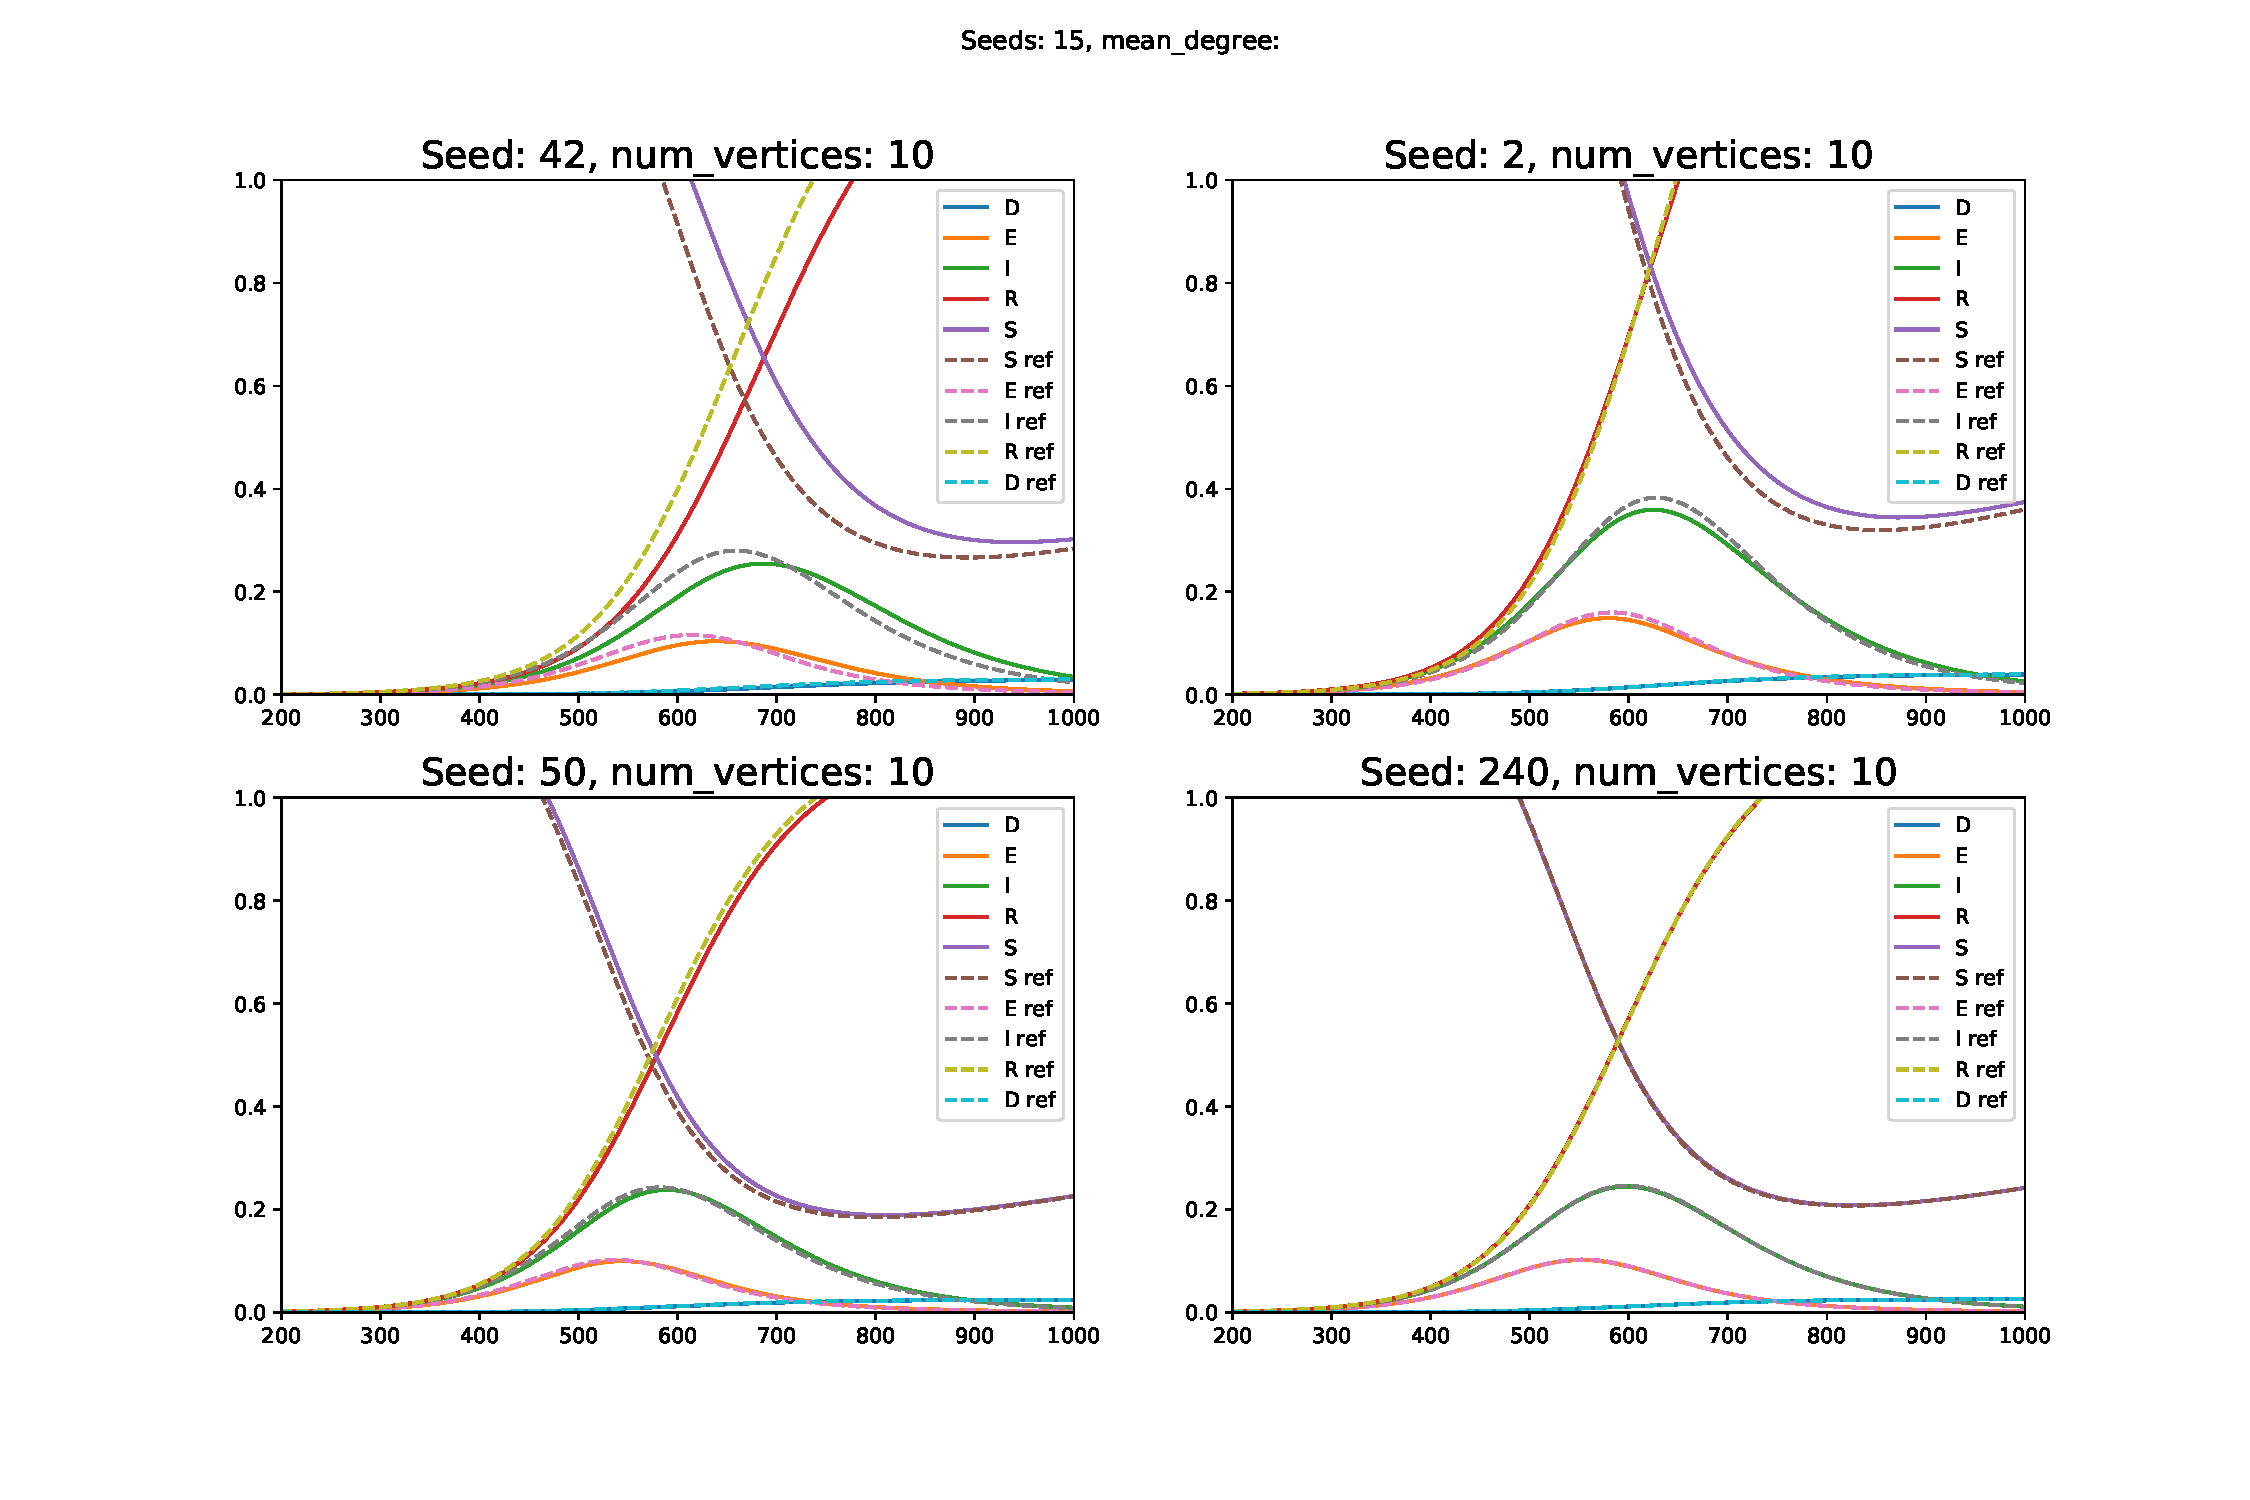
\includegraphics[width=0.8\linewidth]{Bs_swvert_rinf_rinits_rpop-seedcomp.pdf}
        \caption{Darstellung der ersten Infektionswelle aus dem Gesamtpopulationsplot. $\vertices = 100, \mdeg=2$.
        Standardeinstellungen.}%
        \label{fig:Bs_swvert_rinf_rinits_rpop-seedcomp}
    \end{figure}
\end{frame}

\begin{frame}[t]
    \frametitle{Vergleich Erdos-Renyi und Bollobas-Riordan}
    \begin{columns}
        \begin{column}{0.5\textwidth}
            \begin{figure}[htpb]
                \centering
                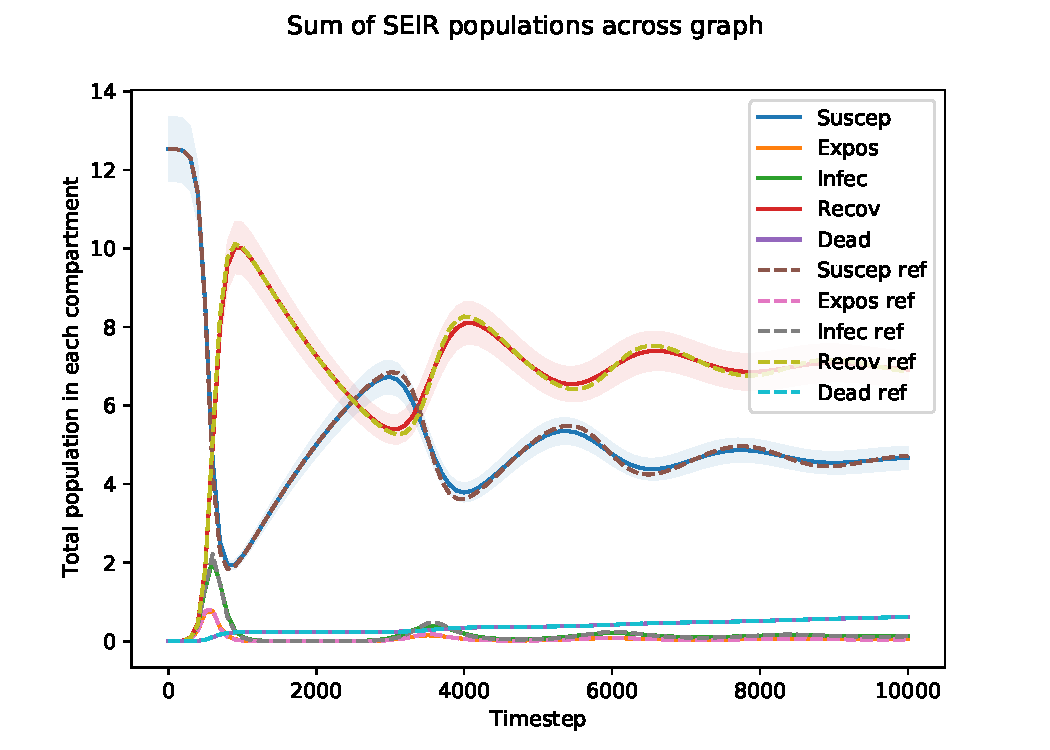
\includegraphics[width=1\linewidth]{ERs_totpop_100-2.pdf}
                \caption{Erdos-Renyi mit $\vertices = 100, \mdeg = 2$.
                Standardeinstellungen.}%
                \label{fig:ERs_totpop_100-2}
            \end{figure}
        \end{column}
        \begin{column}{0.5\textwidth}
            \begin{figure}[htpb]
                \centering
                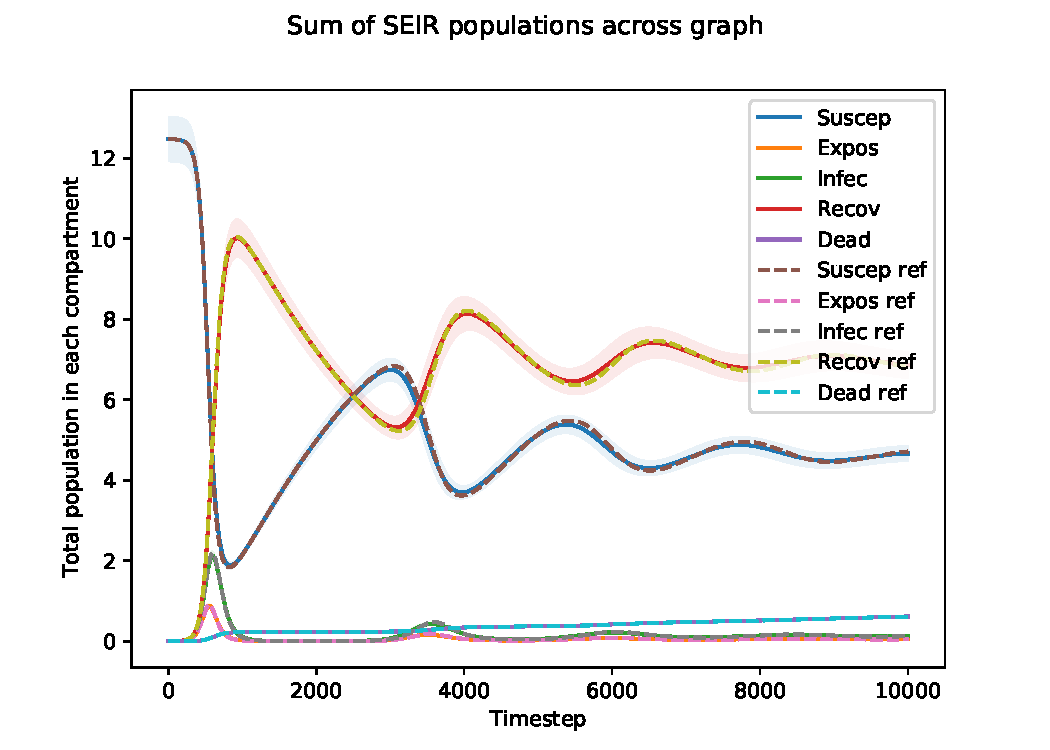
\includegraphics[width=1\linewidth]{bollobas_totpop_seed_100.pdf}
                \caption{Bollobas-Riordan mit $\vertices = 100$.
                Standardeinstellungen.}%
                \label{fig:bollobas_totpop_seed_100}
            \end{figure}
        \end{column}
    \end{columns}
\end{frame}

\section{Stabilität des Modells}
\begin{frame}[t]
    \frametitle{Stabilität des Modells}
    \begin{itemize}
        \item Differentialgleichung dominiert Graphenmodell
        \item Simulation läuft recht zügig in Fixpunkt der DGL
    \end{itemize}
    \begin{columns}
        \begin{column}{0.5\textwidth}
    \begin{figure}[htpb]
        \centering
        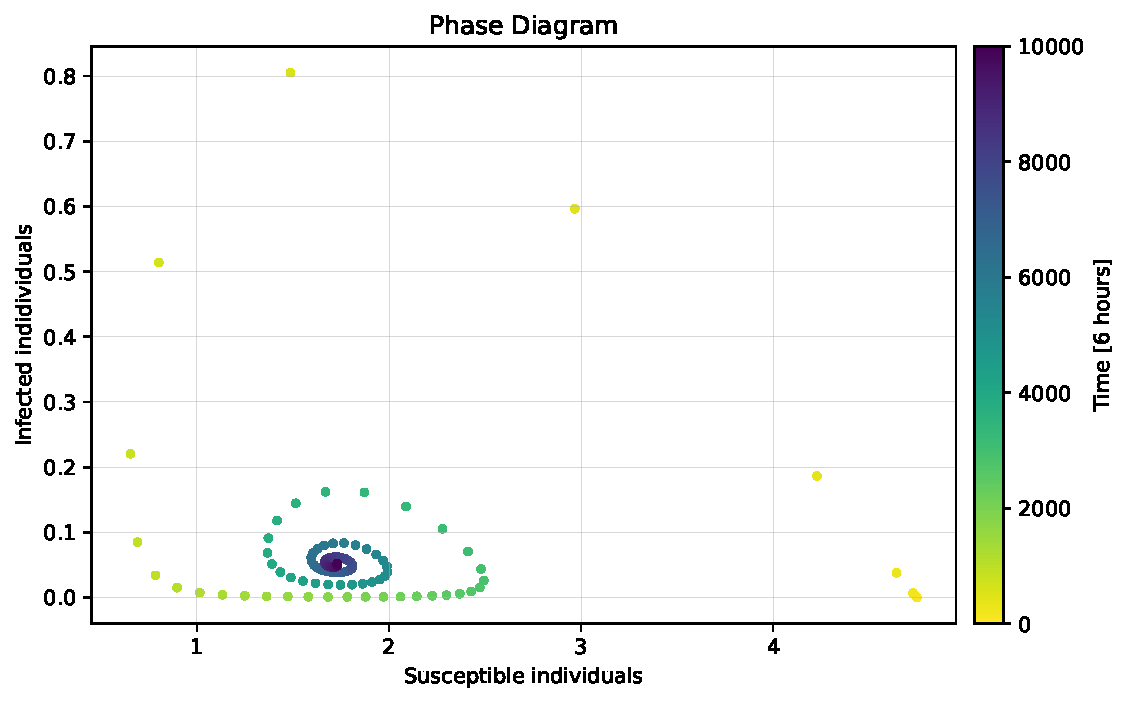
\includegraphics[width=1\linewidth]{ER_SI_phase.pdf}
        \caption{Suszeptible-Infektiöse Phasendiagram für Erdos-Renyi mit $\vertices = 40, \mdeg=2$. Standardeinstellungen.}%
        \label{fig:ER_SI_phase}
    \end{figure}
\end{column}
\begin{column}{0.5\textwidth}
    \begin{figure}[htpb]
        \centering
        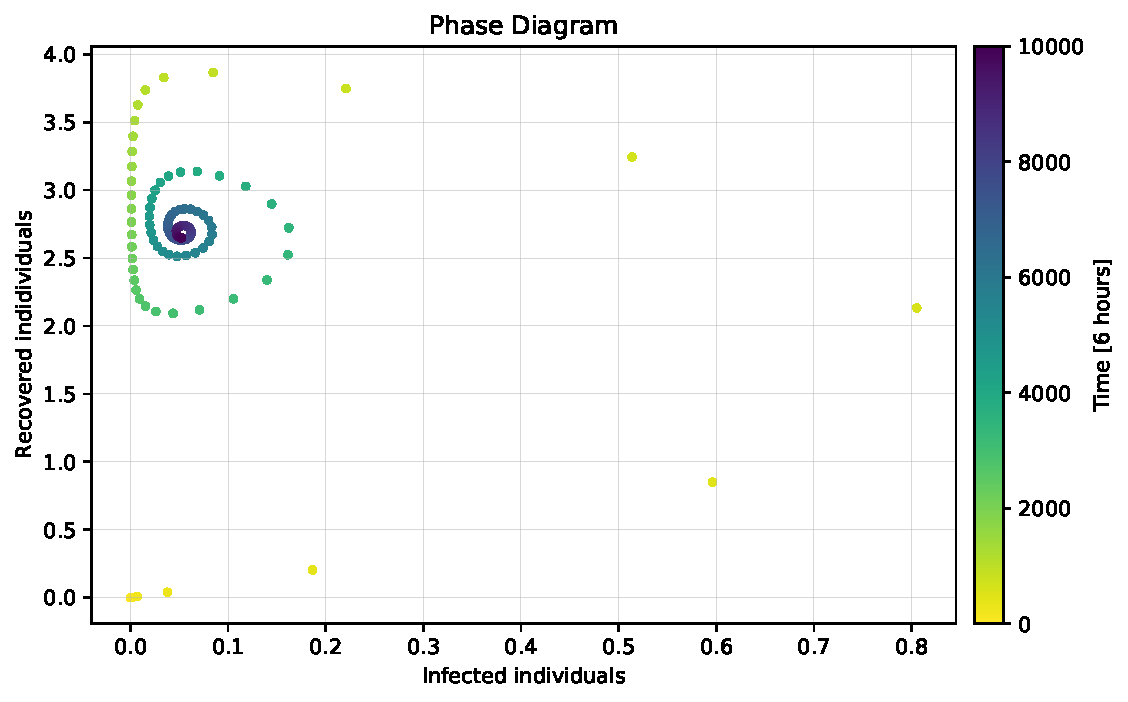
\includegraphics[width=1\linewidth]{ER_IR_phase.pdf}
        \caption{Infektiöse-Recovered Phasendiagram für Erdos-Renyi mit $\vertices = 40, \mdeg=2$.
        Standardeinstellungen.}%
        \label{fig:ER_IR_phase}
    \end{figure}
\end{column}
\end{columns}
\begin{itemize}
    \item<2-> Beobachtbar für jede Parameterkonstellation.
\end{itemize}
\end{frame}
\begin{frame}[t]
    \frametitle{Invertierte Anfangsbedingungen}
    \begin{itemize}
        \item Population startet im immunen Zustand
        \item Sukzessive geht Immunität verloren
    \end{itemize}
    \begin{figure}[htpb]
        \centering
        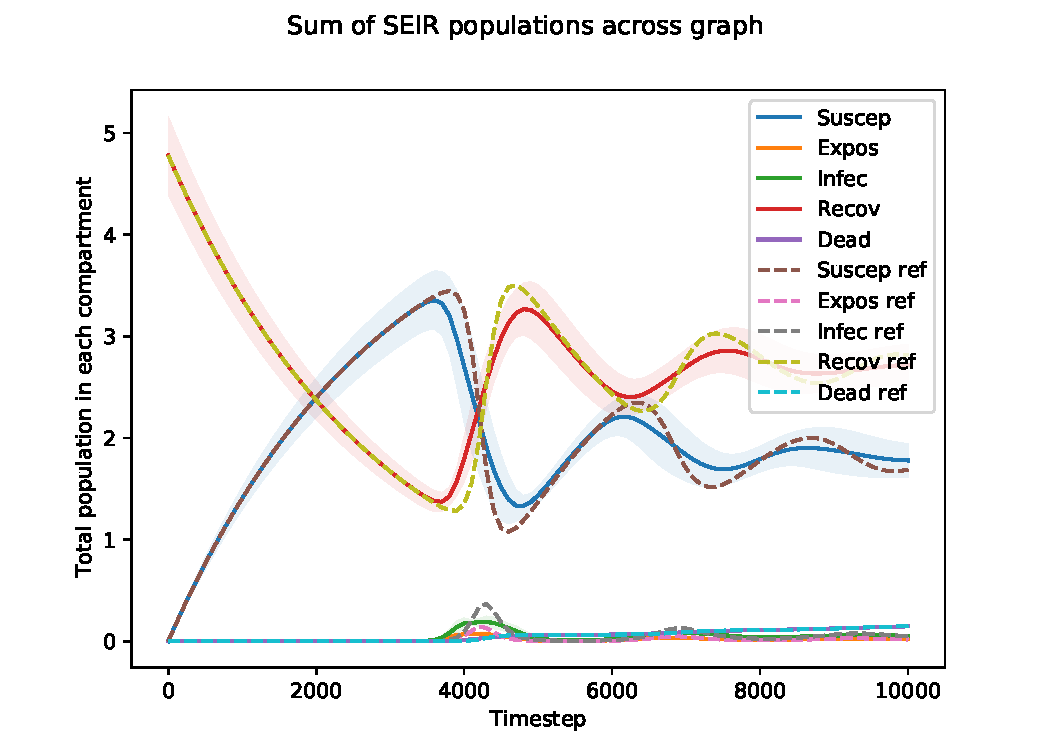
\includegraphics[width=0.7\linewidth]{reversed_init_pop.pdf}
        \caption{Erdos-Renyi mit $\vertices = 40, \mdeg =2$}%
        \label{fig:reversed_init_pop}
    \end{figure}
    
\end{frame}

\begin{frame}[t]
    \frametitle{Variierte Initialisierung der Kantengewichte}
    \begin{figure}[htpb]
        \centering
        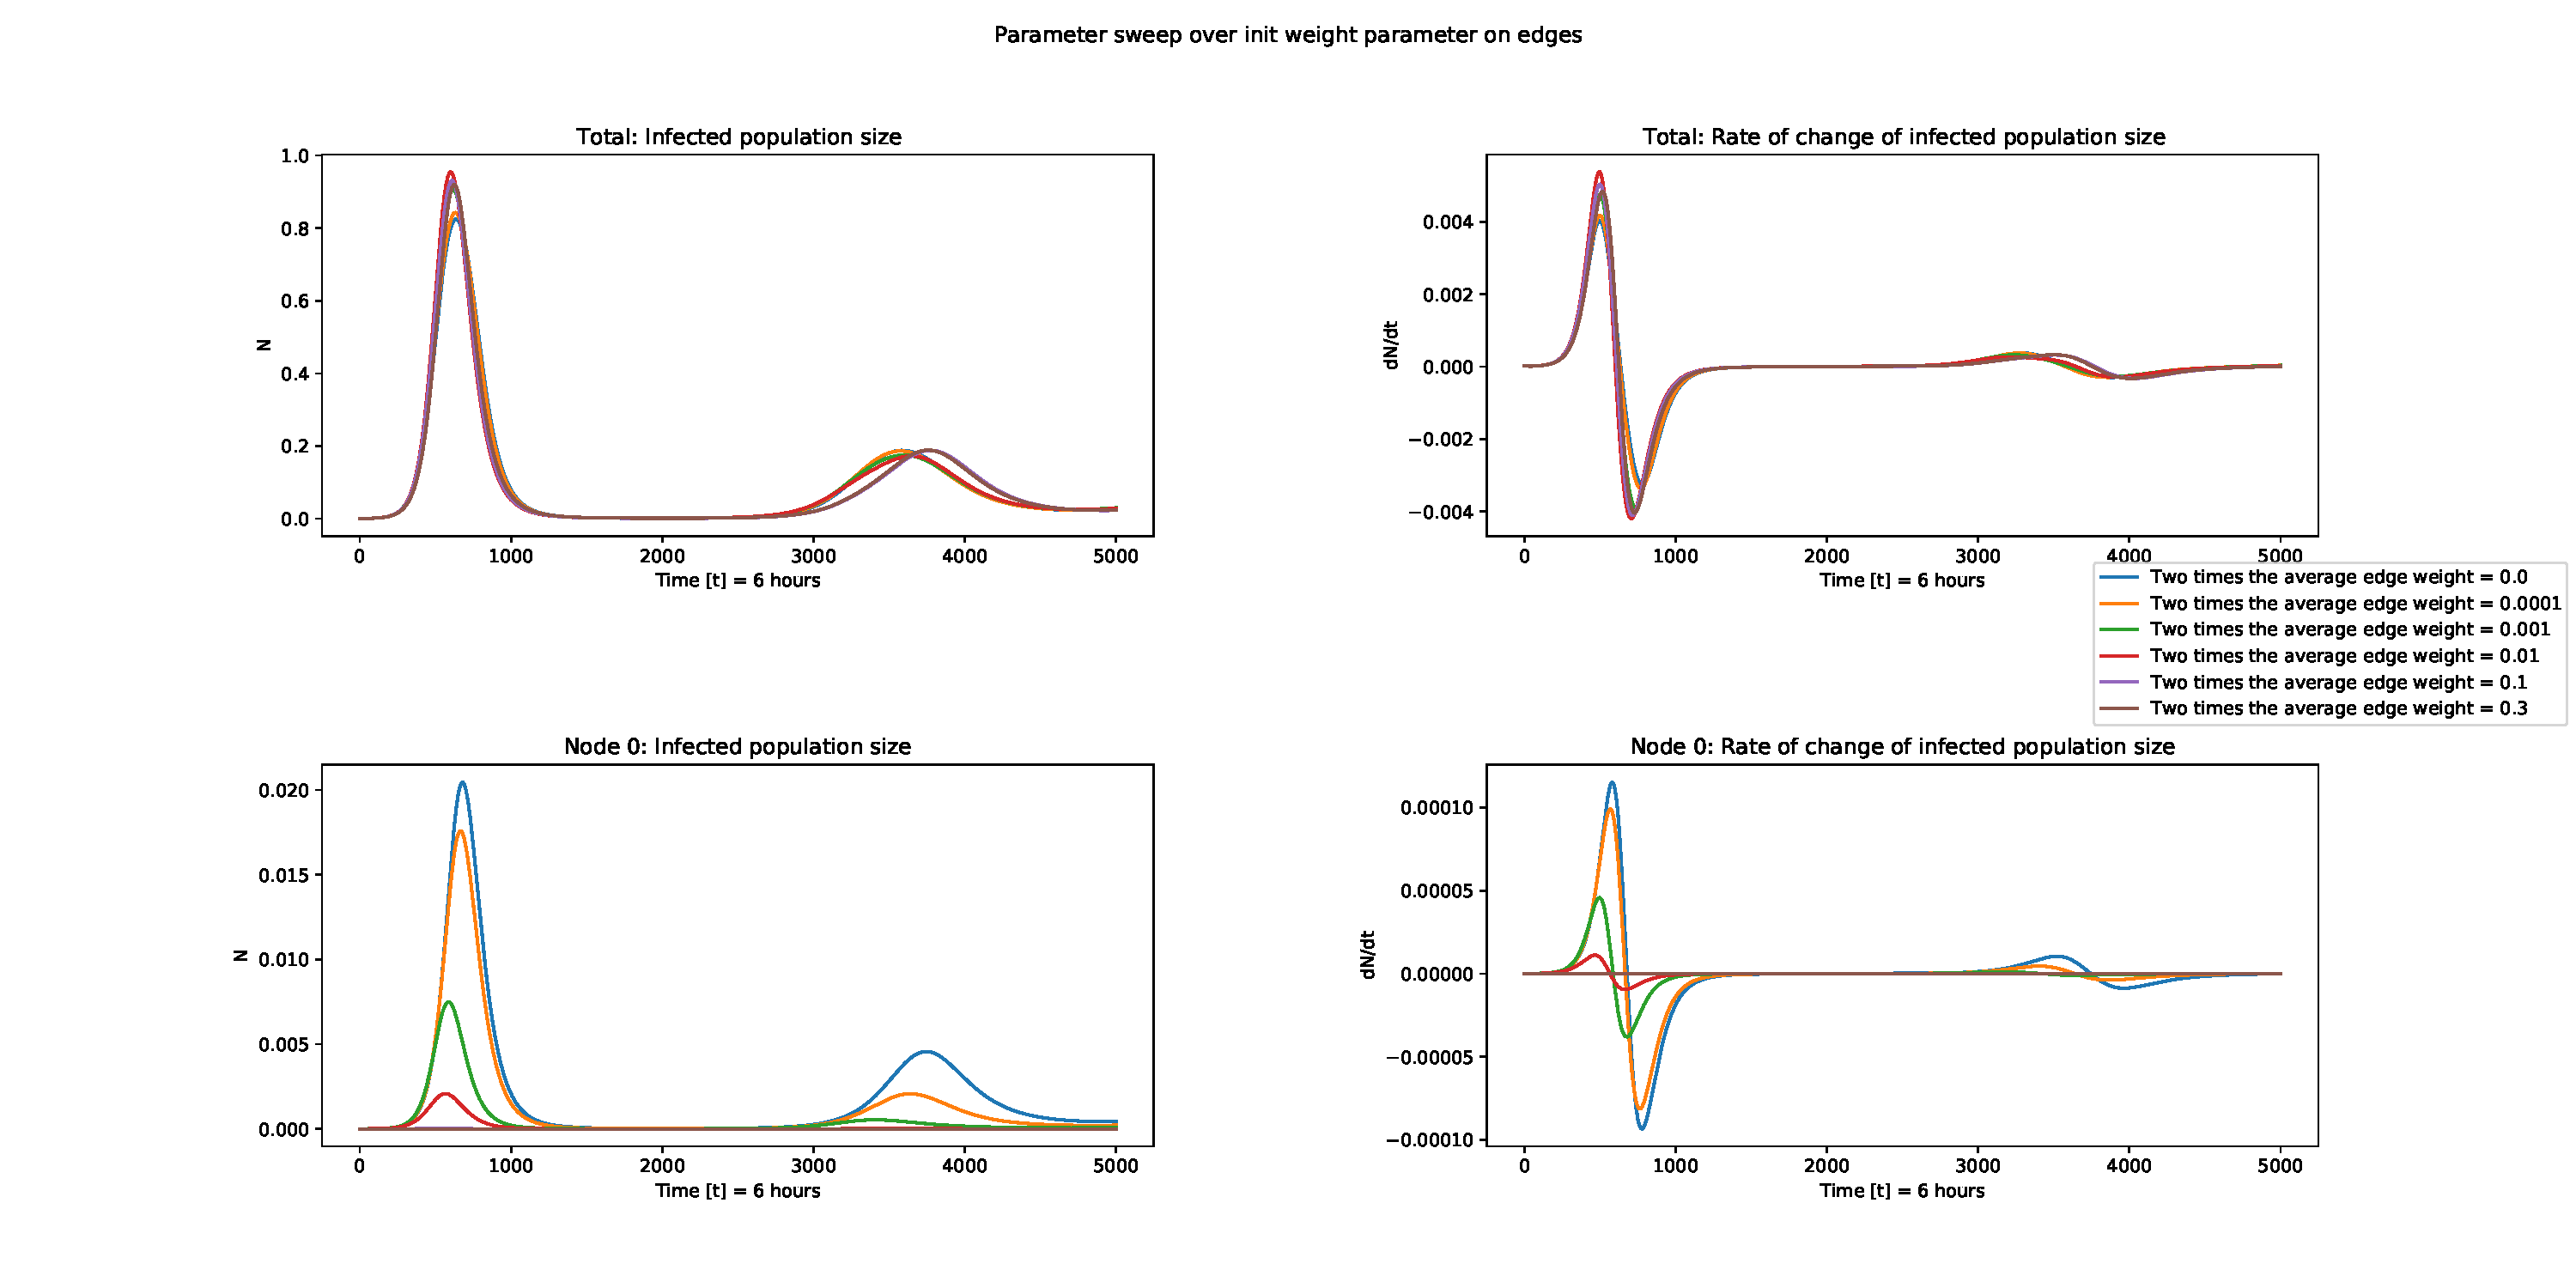
\includegraphics[width=1\linewidth]{init_weight_sweep.pdf}
        \caption{Erdos-Renyi für $\vertices = 40, \mdeg=2$. Standardeinstellungen.}%
        \label{fig:init_weight_sweep}
    \end{figure}
\end{frame}
\begin{frame}[t]
\frametitle{Variierte Initialisierung der Kantengewichte}
Vergleich der Infektionswellen (Proz. Abweichung: $I_{max}, T_{max}$):
    \begin{figure}[htpb]
        \centering
        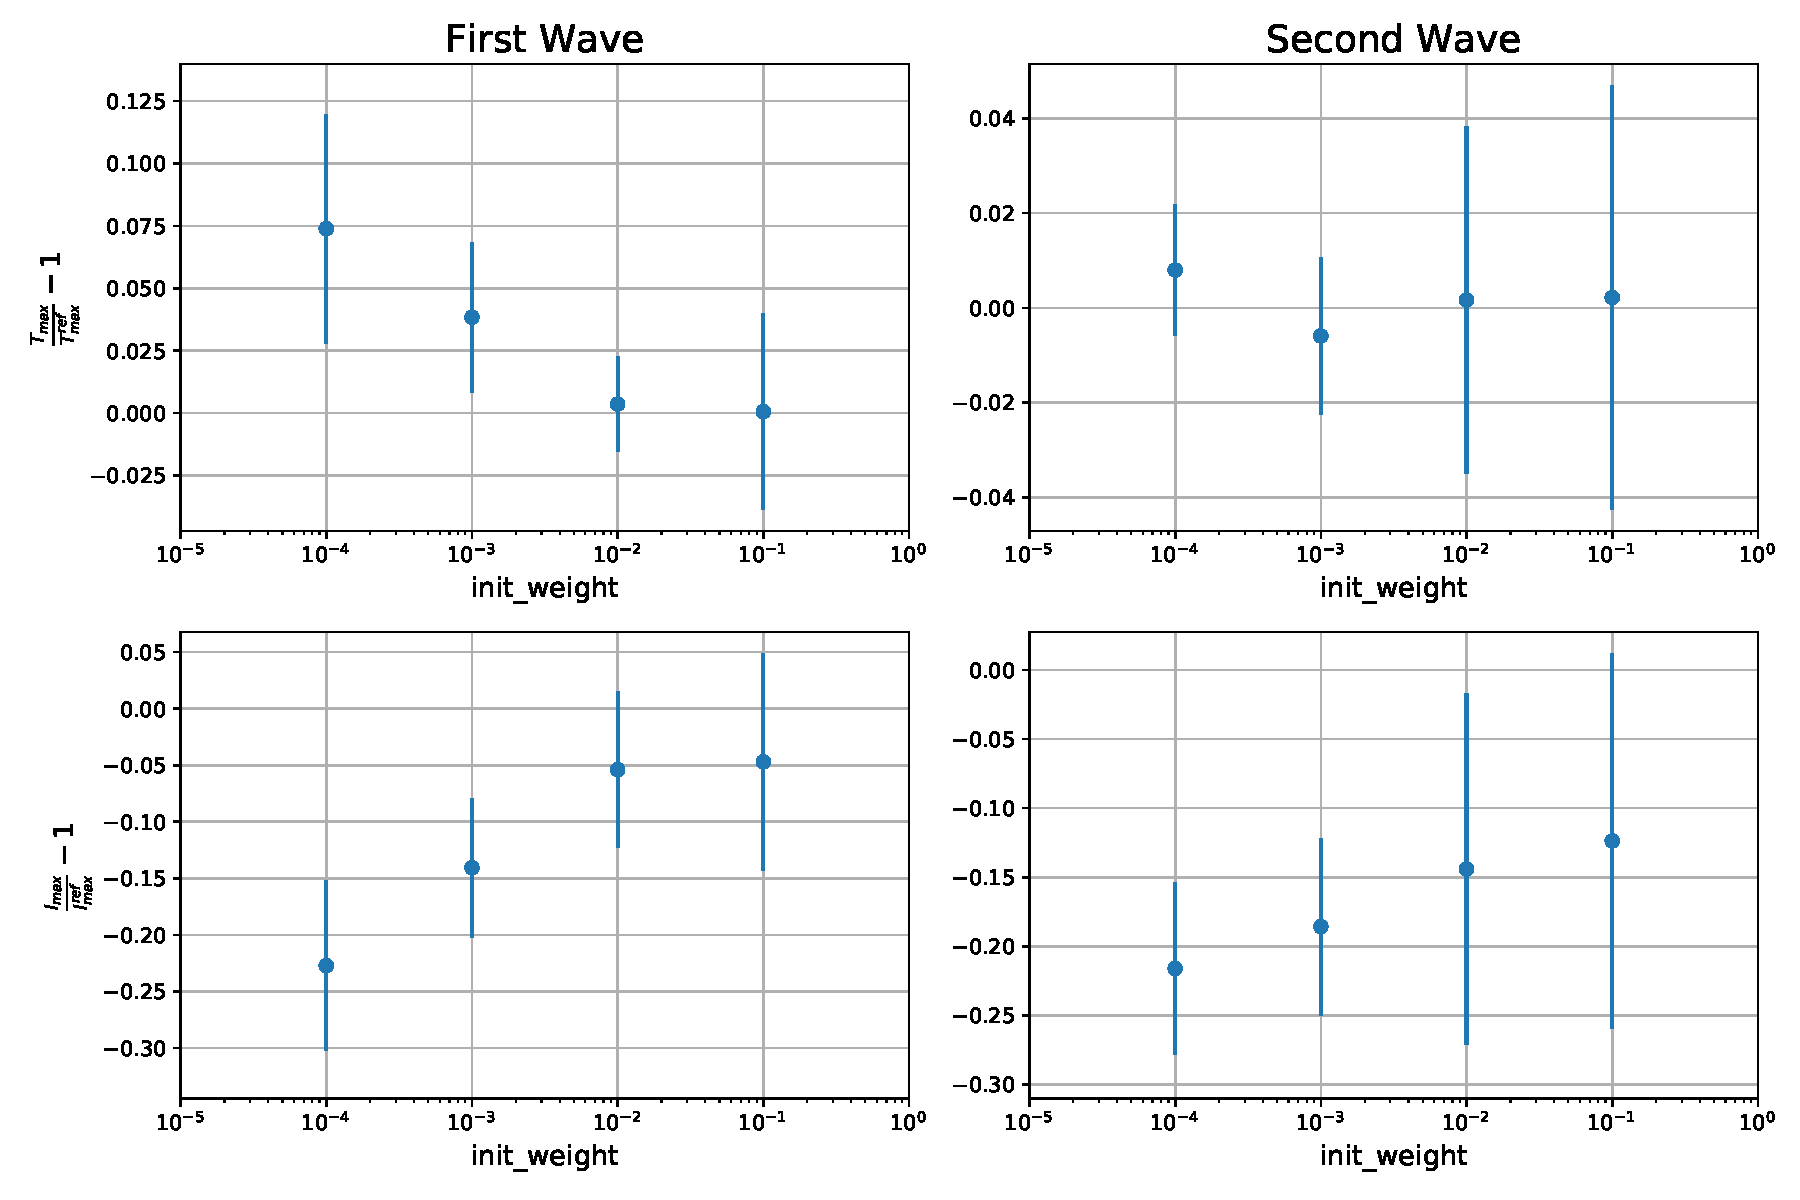
\includegraphics[width=0.8\linewidth]{ERs_swinit_weight_rinf_rinits_rpop-wavecomp.pdf}
        \caption{Erdos-Renyi mit $\vertices = 50, \mdeg=2$. Standardeinstellung mit variierter
        Initialisierung der Kantengewichte.}% 
        \label{fig:ERs_swinit_weight_rinf_rinits_rpop-wavecomp}
    \end{figure}
\end{frame}
\begin{frame}[t]
    \frametitle{Variierte Mobilität von Infizierten}
    \begin{columns}
        \begin{column}{0.5\textwidth}
            \begin{figure}[htpb]
                \centering
                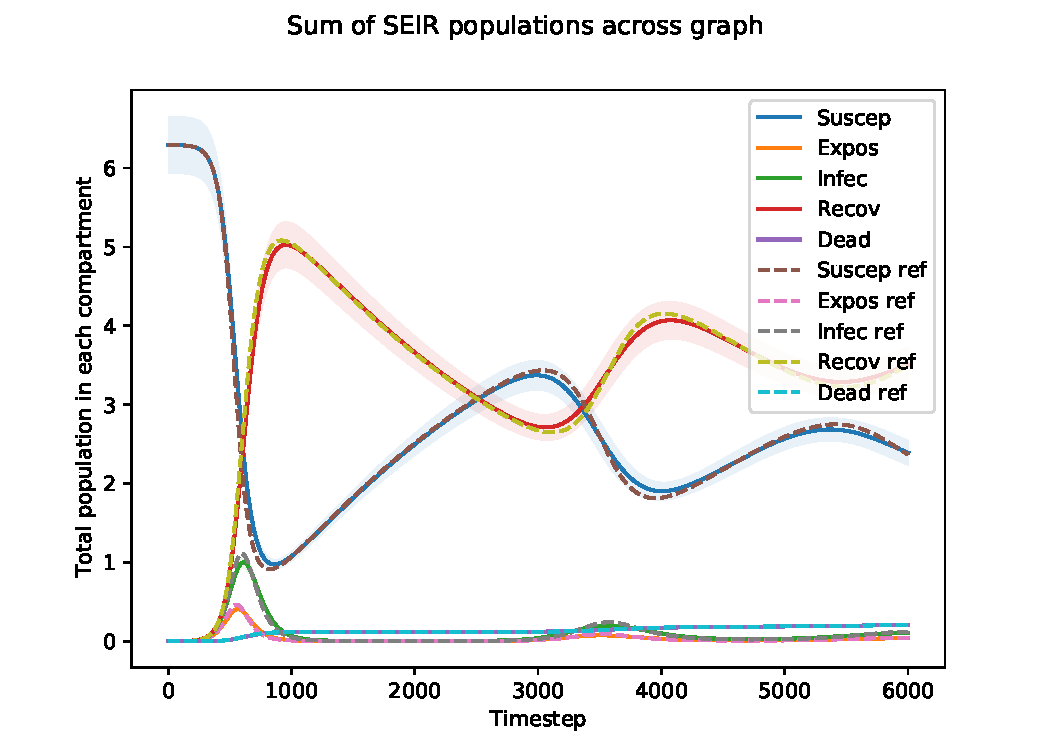
\includegraphics[width=0.8\linewidth]{ERs_swi_weight_totpop.pdf}
                \caption{Erdos-Renyi mit $\vertices=50, \mdeg=2$ und \emph{i\_weight}$=0.1$.}%
                \label{fig:ERs_swi_weight_totpop}
            \end{figure}
        \end{column}
        \begin{column}{0.5\textwidth}
            \begin{figure}[htpb]
                \centering
                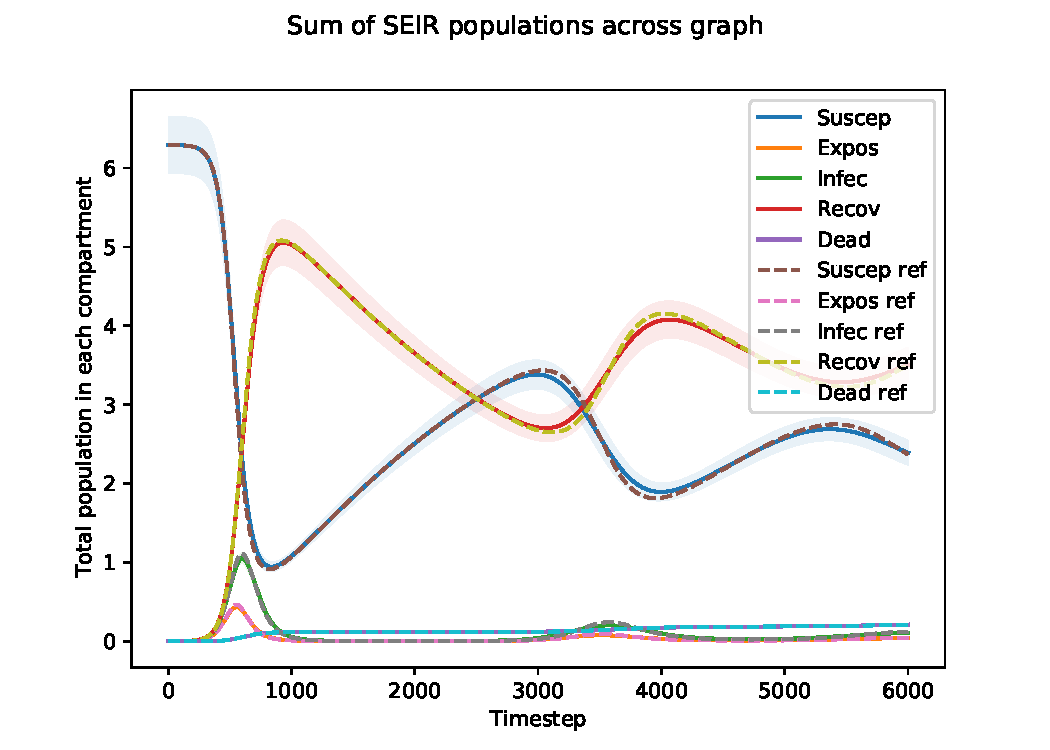
\includegraphics[width=0.8\linewidth]{ERs_swi_weight_totpop_1.pdf}
                \caption{Erdos-Renyi mit $\vertices=50, \mdeg=2$ und \emph{i\_weight} $=0.5$.}%
                \label{fig:ERs_swi_weight_totpop_05}
            \end{figure}
        \end{column}
    \end{columns}
    \begin{itemize}
        \item Eingeschränkte Mobilität von Infizierten lässt Dynamik im Wesentlichen unverändert
        \item Leichte Abweichungen zu Referenzmodell sind beobachtbar
    \end{itemize}
\end{frame}

\begin{frame}[t]
    \frametitle{Variierte Mobilität von Infizierten}
    Vergleich der Infektionswellen (Proz. Abweichung: $I_{max}, T_{max}$):
    \begin{figure}[htpb]
        \centering
        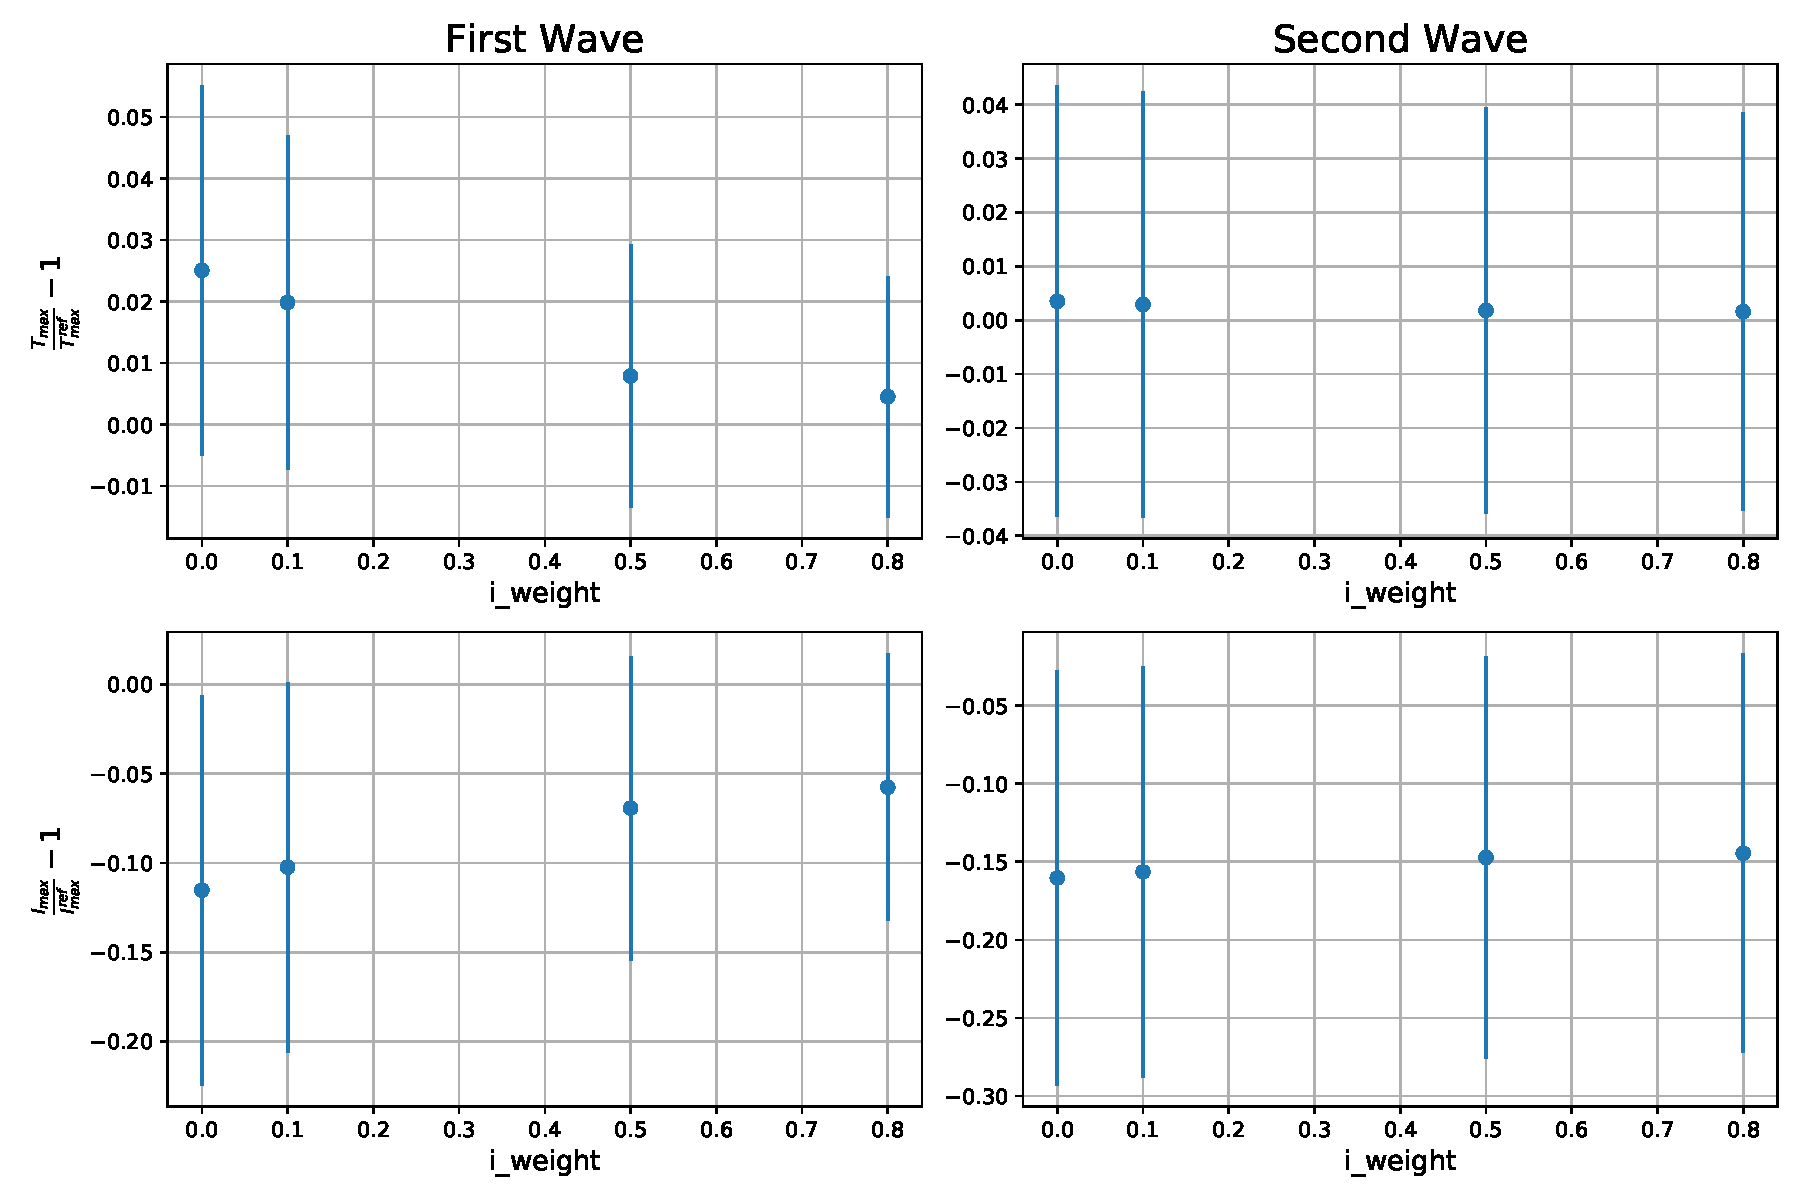
\includegraphics[width=0.8\linewidth]{ERs_swinf_weight_rinf_rinits_rpop-wavecomp.pdf}
        \caption{Erdos-Renyi für $\vertices = 50, \mdeg=2$. Standardeinstellungen mit Sweep über die
        Gewichtung der Infizierten.}%
        \label{fig:ERs_swinf_weight_rinf_rinits_rpop-wavecomp}
    \end{figure}
    
\end{frame}
